\newcommand{\DoNotLoadEpstopdf}{}
\documentclass[11pt,letterpaper]{article}
\usepackage[T1]{fontenc}
\usepackage[utf8]{inputenc}
\usepackage[margin=.83in,top=.82in,bottom=.83in,headheight=23pt,headsep=.19in]{geometry}
\usepackage{amsmath,amssymb,amsthm,mathtools}
\usepackage{mathpazo,helvet,microtype}
\usepackage{booktabs,tabularx,array,longtable}
\usepackage{graphicx,xcolor,tikz}
\usetikzlibrary{arrows.meta,positioning,calc,fit,backgrounds}
\usepackage[most]{tcolorbox}
\usepackage{enumitem,needspace,fancyhdr,titlesec,caption,float,placeins}
\usepackage{etoolbox}
\usepackage{listings,xurl,upquote}
\usepackage[numbers,sort&compress]{natbib}
\usepackage[unicode,bookmarksnumbered]{hyperref}
\usepackage{bookmark}
\definecolor{Ink}{HTML}{201529}
\definecolor{Plum}{HTML}{482A50}
\definecolor{Wine}{HTML}{772F52}
\definecolor{Gold}{HTML}{A5772D}
\definecolor{LightGold}{HTML}{EDCE8B}
\definecolor{Ivory}{HTML}{FCF9F2}
\definecolor{Teal}{HTML}{146D68}
\definecolor{Mint}{HTML}{B6E6D7}
\definecolor{Muted}{HTML}{655F6A}
\definecolor{Rule}{HTML}{D9CFC1}
\definecolor{Pale}{HTML}{F3EEF5}
\hypersetup{pdftitle={LEARNING TO BUILD: How Intelligence Learns to Create What Makes New Possibilities Real},pdfauthor={Vincent Boucher},pdfsubject={Complete productive means, construction learning, and the expansion of attainable possibilities},pdfkeywords={Transformational Intelligence, Learning to Build, Alpha Genesis Flywheel, construction frontier, capability construction, learning, productive capacity},colorlinks=true,linkcolor=Plum,citecolor=Plum,urlcolor=Teal}
\ifdefined\pdfinfoomitdate\pdfinfoomitdate=1\fi
\ifdefined\pdftrailerid\pdftrailerid{}\fi
\ifdefined\pdfsuppressptexinfo\pdfsuppressptexinfo=15\fi
\pagestyle{fancy}\fancyhf{}
\fancyhead[L]{\footnotesize\sffamily\color{Muted}LEARNING TO BUILD}
\fancyhead[R]{\footnotesize\sffamily\color{Muted}Boucher\;|\;Research edition 1.1.0}
\fancyfoot[L]{\scriptsize\sffamily\color{Muted}TRANSFORMATIONAL INTELLIGENCE $\infty$}
\fancyfoot[R]{\small\color{Gold}\thepage}
\renewcommand{\headrulewidth}{.35pt}
\renewcommand{\headrule}{\hbox to\headwidth{\color{Rule}\leaders\hrule height \headrulewidth\hfill}}
\setlength{\parindent}{0pt}\setlength{\parskip}{.46em plus .07em minus .04em}
\setlength{\emergencystretch}{2.8em}\linespread{1.035}\raggedbottom
\widowpenalty=10000\clubpenalty=10000
\titleformat{\section}{\Large\bfseries\color{Plum}}{\color{Gold}\thesection}{.65em}{}
\titleformat{\subsection}{\large\bfseries\color{Ink}}{\thesubsection}{.65em}{}
\titleformat{\subsubsection}{\normalsize\bfseries\color{Ink}}{\thesubsubsection}{.65em}{}
\titlespacing*{\section}{0pt}{2.2ex plus .4ex minus .2ex}{.8ex}
\titlespacing*{\subsection}{0pt}{1.6ex plus .3ex minus .2ex}{.5ex}
\preto\section{\Needspace{7\baselineskip}}
\preto\subsection{\Needspace{5\baselineskip}}
\captionsetup{font=small,labelfont={bf,color=Plum},textfont={color=Muted},skip=7pt}
\setlist{leftmargin=1.45em,itemsep=.18em,topsep=.25em,parsep=0pt}
\renewcommand{\arraystretch}{1.15}
\newcolumntype{Y}{>{\raggedright\arraybackslash}X}
\newcolumntype{P}[1]{>{\raggedright\arraybackslash}p{#1}}
\newcommand{\E}{\mathbb{E}}\newcommand{\Prob}{\mathbb{P}}
\newcommand{\I}{\mathcal{I}}\newcommand{\M}{\mathcal{M}}\newcommand{\K}{\mathcal{K}}
\newcommand{\R}{\mathcal{R}}\newcommand{\C}{\mathcal{C}}\newcommand{\F}{\mathcal{F}}
\DeclareMathOperator*{\argmax}{arg\,max}
\DeclareMathOperator*{\argmin}{arg\,min}
\newtheorem{definition}{Definition}[section]
\newtheorem{proposition}{Proposition}[section]
\newtheorem{corollary}{Corollary}[section]
\theoremstyle{remark}\newtheorem{remark}{Remark}[section]
\newtcolorbox{thesisbox}{enhanced,breakable,colback=Ivory,colframe=Gold,boxrule=.5pt,arc=1.3mm,left=12pt,right=12pt,top=10pt,bottom=10pt,before skip=10pt,after skip=10pt}
\newtcolorbox{statusbox}{enhanced,breakable,colback=Pale,colframe=Plum,boxrule=0pt,borderline west={2.5pt}{0pt}{Plum},arc=0mm,left=11pt,right=11pt,top=8pt,bottom=8pt,before skip=9pt,after skip=9pt}
\newtcolorbox{practicebox}{enhanced,breakable,colback=Teal!5,colframe=Teal,boxrule=0pt,borderline west={2.5pt}{0pt}{Teal},arc=0mm,left=11pt,right=11pt,top=8pt,bottom=8pt,before skip=9pt,after skip=9pt}
\newcommand{\smallhead}[1]{\par\smallskip{\sffamily\bfseries\color{Gold}#1}\par\smallskip}
\lstset{upquote=true,basicstyle=\small\ttfamily,breaklines=true,columns=fullflexible,keepspaces=true,showstringspaces=false,frame=single,rulecolor=\color{Rule},backgroundcolor=\color{Ivory},framesep=7pt}
\setcounter{tocdepth}{1}
\begin{document}
\begin{titlepage}
\thispagestyle{empty}

\begin{tikzpicture}[remember picture,overlay]
\fill[Ink] (current page.south west) rectangle (current page.north east);
\fill[Plum,opacity=.6] ([yshift=2.45in]current page.south west) rectangle ([yshift=-4.45in]current page.north east);
\draw[LightGold,opacity=.65,line width=.6pt] ([xshift=.34in,yshift=.34in]current page.south west) rectangle ([xshift=-.34in,yshift=-.34in]current page.north east);
\node[anchor=north west,text=LightGold,font=\sffamily\small] at ([xshift=.72in,yshift=-.64in]current page.north west) {MONTREAL.AI\quad /\quad QUEBEC.AI};
\node[anchor=north east,text=LightGold,font=\sffamily\small] at ([xshift=-.72in,yshift=-.64in]current page.north east) {RESEARCH 1.1.0};
\node[anchor=north,text=Ivory,font=\sffamily\fontsize{14}{19}\selectfont] at ([yshift=-1.33in]current page.north) {TRANSFORMATIONAL INTELLIGENCE $\infty$};
\node[anchor=north,text=Ivory,font=\fontsize{43}{48}\selectfont\bfseries] at ([yshift=-1.94in]current page.north) {LEARNING};
\node[anchor=north,text=LightGold,font=\fontsize{58}{64}\selectfont\bfseries] at ([yshift=-2.66in]current page.north) {TO BUILD};
\node[anchor=north,align=center,text=Ivory,text width=6.6in,font=\fontsize{16}{22}\selectfont] at ([yshift=-3.81in]current page.north) {How Intelligence Learns to Create\\What Makes New Possibilities Real};
\begin{scope}[shift={([xshift=.93in,yshift=3.32in]current page.south west)},x=1in,y=1in]
% An original vector construction: each platform supports a further platform.
\foreach \y in {0,.2,.4,.6,.8,1,1.2,1.4,1.6,1.8,2}{\draw[Mint,opacity=.06,line width=.3pt] (0,\y)--(6.6,\y);}
\foreach \x in {0,.3,...,6.6}{\draw[Mint,opacity=.05,line width=.3pt] (\x,-.1)--(\x,2.2);}
\draw[LightGold,opacity=.75,line width=1.1pt] (.2,0)--(6.4,0);
\foreach \x/\h in {.55/.45,1.55/.8,2.55/1.15,3.55/1.5,4.55/1.85}{
 \draw[LightGold,line width=.9pt] (\x,0)--(\x,\h)--++(.8,0);
 \draw[LightGold,opacity=.45,line width=.6pt] (\x,0)--(\x+.8,\h);
 \draw[LightGold,opacity=.45,line width=.6pt] (\x+.8,0)--(\x,\h);
 \draw[LightGold,line width=.6pt] (\x+.8,0)--(\x+.8,\h);
 \fill[LightGold] (\x,\h) circle(1.9pt);
}
\draw[Mint,line width=1.1pt,-{Latex[length=2.5mm]}] (1.16,.57) .. controls (2.0,1.3) and (4.0,1.58) .. (5.77,2.28);
\draw[LightGold,line width=.8pt] (5.7,1.85)--(5.7,2.6)--(4.55,2.6)--(6.33,2.6);
\draw[LightGold,line width=.5pt] (5.7,2.9)--(4.55,2.6) (5.7,2.9)--(6.33,2.6) (5.7,2.9)--(5.7,2.6);
\draw[LightGold,line width=.5pt] (6.12,2.6)--(6.12,2.12);
\draw[Mint,line width=1.1pt] (5.98,2.1)--(6.26,2.1)--(6.26,1.93)--(5.98,1.93)--cycle;
\node[text=Mint,font=\fontsize{39}{43}\selectfont] at (1.15,1.95) {$\infty$};
\fill[LightGold] (3.55,2.45)--(3.59,2.57)--(3.63,2.45)--(3.75,2.41)--(3.63,2.37)--(3.59,2.25)--(3.55,2.37)--(3.43,2.41)--cycle;
\end{scope}
\node[anchor=north,align=center,text=Ivory,text width=6.7in,font=\fontsize{17}{23}\selectfont] at ([yshift=-8.05in]current page.north) {When we build something new,\\\textcolor{LightGold}{we change what can be built next.}};
\node[anchor=south west,text=Ivory,align=left,font=\normalsize] at ([xshift=.72in,yshift=.76in]current page.south west) {\textbf{Vincent Boucher}\\Montr\'{e}al, Qu\'{e}bec, Canada};
\node[anchor=south east,text=LightGold,align=right,font=\small] at ([xshift=-.72in,yshift=.76in]current page.south east) {ALPHA GENESIS FLYWHEEL $\Omega$\\7 November 2026};
\end{tikzpicture}
\null
\end{titlepage}

\setcounter{page}{1}
\begin{center}
{\small\sffamily\bfseries\color{Gold}ALPHA GENESIS FLYWHEEL $\Omega$}\par\vspace{.12in}
{\LARGE\bfseries\color{Plum}LEARNING TO BUILD}\par\vspace{.1in}
{\Large How Intelligence Learns to Create\\What Makes New Possibilities Real}\par\vspace{.16in}
\textbf{Vincent Boucher}\quad$\cdot$\quad MONTREAL.AI / QUEBEC.AI\\
{\small Montr\'{e}al, Qu\'{e}bec, Canada\quad$\cdot$\quad 7 November 2026}
\end{center}
\smallhead{ABSTRACT}
A useful idea can remain unrealizable because its necessary knowledge, instruments, processes, resources, and arrangements do not yet work together. We develop an operational account of \emph{learning to build}: constructing these complete, purpose-relative means and testing whether experience improves the construction of fresh means. The contribution is a linked representation and evaluation discipline. A construction witness connects an executable policy to its interfaces, resource schedule, authority, evidence, and continuing obligations; installed and construction frontiers separate what can be operated now from what can be made attainable; and transfer controls separate an inherited artifact, a revised constructor, and a better construction-learning rule. The account joins \emph{Transformational Intelligence}, \emph{Invent the Economy}, and \emph{ALPHA GENESIS FLYWHEEL $\Omega$}, while building on systems engineering, program learning, and economic complementarity. The preserved 1.0.0 illustration emits four programs that pass 4,000 finite input checks; a conventional equal-content planner ties all 288 authored resource scenarios. This edition adds a registered microscopy construction and a reproduction of its exposed comparison: nucleus analysis, a whole-cell successor with a distinct acceptance boundary, six classical construction arms with a shared candidate bank, and a separately identified pretrained specialist. The pretrained nucleus instrument meets every source research gate on both cohorts; its whole-cell successor fails the boundary gate (test F1 0.506 versus the required 0.60). The classical nucleus instrument fails its validation count-error gate; all six classical successor arms exhaust the 24-recipe bank, select the same unqualified instrument, and tie in candidate executions. Frozen order replays explain this convergence, and a separately frozen foreground composition fails calibration. Successful operation, successor qualification, constructor advantage, and funded continuation remain separate verdicts. The empirical scope is a public-image research instrument and a finite supplied recipe bank. It does not establish autonomous open-ended invention, newly learned segmentation algorithms, laboratory acceptance, or earned commercial continuation. The long-term hypothesis is that useful constructions can create both productive means and transferable methods for building the next set of means; each link requires its own evidence.
\begin{statusbox}
\textbf{Research edition 1.1.0.} A conceptual synthesis, elementary conditional results, the preserved 1.0.0 computational illustration, and a versioned microscopy continuation. The new execution is a reproduction of an already exposed registered comparison, not a newly concealed confirmation task. Measured conclusions and their source boundary are stated in Section~\ref{sec:continuation}. The published 1.0.0 source and evidence remain available unchanged.
\end{statusbox}
{\small\textbf{Keywords:} transformational intelligence; complete means; capability construction; construction learning; complementary capabilities; successor evaluation; productive capacity.}
\clearpage
\section*{The idea in one minute}
\addcontentsline{toc}{section}{The idea in one minute}

A promising experiment, process, or service may lack one necessary ability. Learning to build asks: \emph{can we construct its complete means, and does that experience make us better at a different construction?}

\begin{thesisbox}
\textbf{The proposed unit of progress is an accepted change in what someone can do, with an account of its construction and continuing requirements.}
\end{thesisbox}

\smallhead{FOUR CLAIMS, FOUR TESTS}
\begin{tabularx}{\linewidth}{@{}P{1.5in}Y@{}}
\toprule
\textbf{Claim} & \textbf{Evidence it needs}\\
\midrule
A useful construction & An operating instrument meets its declared acceptance boundary.\\
A useful inheritance & Retained means help a different accepted outcome after adaptation and support costs.\\
A better constructor & A revised procedure beats a strong method given the same legitimate content and resources.\\
A better learning rule & The rule improves constructors across independent development and confirmation campaigns.\\
\bottomrule
\end{tabularx}

\smallhead{WHAT THIS EDITION CONTRIBUTES}
\textbf{A conceptual connection.} Complete means, an executable witness, resource and authority prefixes, continuing obligations, and successor tests form one account of construction learning. The contribution connects established components around a specific object of learning and a falsifiable attribution test.

\textbf{Two evidence boundaries.} The preserved 1.0.0 illustration uses a finite authored model. This continuation builds public-image microscopy instruments, compares a supplied ordering update with ordinary empirical ranking, and evaluates a separately registered pretrained specialist.

\textbf{The measured result.} The pretrained nucleus route qualifies for the research contract; its whole-cell successor fails. The classical source and successor also fail. All six classical arms exhaust the recipe bank and tie. No accepted constructor advantage is established.

\textbf{The claim boundary.} A useful tool does not prove a better builder. Benchmark operation does not establish laboratory acceptance, commercial demand, or a self-sustaining enterprise.

\begin{practicebox}
\textbf{Start with one useful outcome.} Name its beneficiary and missing means. Compare the strongest complete existing route, build a decisive artifact, and test a fresh successor with the finished donor artifact withheld where required. Use the brief in Appendix~\ref{app:brief}.
\end{practicebox}

\textbf{Reading routes.} Idea: Section~\ref{sec:opening}. Model: Sections~\ref{sec:means}--\ref{sec:builder}. Microscopy: Section~\ref{sec:continuation}. Research design: Section~\ref{sec:evaluation}. Begin: Section~\ref{sec:programme}. Reproduce: Appendix~\ref{app:reproduction}.

\smallhead{EN FRAN\c{C}AIS}
\begingroup\small
\textbf{APPRENDRE \`A CONSTRUIRE}\par
Cr\'eer les moyens qui rendent une possibilit\'e r\'ealisable, puis v\'erifier si l'exp\'erience am\'eliore une construction diff\'erente: tel est l'objectif. Un instrument utile, un transfert r\'eussi et une meilleure m\'ethode sont des r\'esultats distincts. Cette \'edition conserve la version 1.0.0 et ajoute une recherche en microscopie, ses comparaisons et ses limites. Article int\'egral en anglais.
\endgroup

\clearpage
\tableofcontents
\clearpage
\section{The next breakthrough may be the ability to build it}
\label{sec:opening}

Imagine a laboratory that could test an important new material, except that the necessary measurement cannot yet be made reliably. An algorithm can propose the experiment. A designer can draw the apparatus. A manufacturer can make its parts. Yet the useful capability may remain absent: the parts do not interface, calibration is missing, the reference sample is unavailable, or no one can fund the sequence before an accepted result exists. This is an illustrative situation, not an experiment reported in this paper.

The consequential construction is the complete means of performing the measurement. Its output is an ability: someone can now make a distinction, produce a result, or undertake useful work that was previously inaccessible under the stated conditions. The construction can include familiar components. Its significance lies in what they make possible together.

Now consider a second laboratory problem. Keeping the first apparatus may help. Keeping its design principles may help a different apparatus. Learning a better way to identify missing measurements, construct fixtures, diagnose failures, and qualify new designs would be a further achievement. The object that improves has changed from an instrument to the process of making instruments.

\begin{thesisbox}
\textbf{Learning to build is improving the ability to turn a worthwhile possibility into working, accepted means---and to make fresh construction better through what was learned.}
\end{thesisbox}

This is the connective tissue between an ambitious idea and an expanding productive civilization. A useful instrument can improve science. Better science can improve processes. A qualified process can make further instruments, energy systems, or production facilities affordable. Their operation can supply resources and knowledge for another construction. Every connection is a claim to be tested; the sequence is a research and enterprise objective, not an inevitable trajectory.

\subsection{The unit of progress is a changed ability}

An answer is often exactly what is needed. So is an existing tool, a purchased service, or a simple process change. Construction becomes relevant when an important outcome remains blocked because the required means are absent, incompatible, unreliable, or unaffordable. The right response need not be a larger system. It may remove a requirement that belonged only to the old method, or replace an intricate solution with a mature alternative.

The phrase \emph{what makes new possibilities real} therefore has an operational meaning. State an accepted outcome; identify the initial conditions; construct a permitted route; execute and check it at the claimed evidential level. A digital artifact can be a real computational construction. A simulated factory is a model of a factory. A proposed sale is a hypothesis about a relationship. These distinctions preserve the meaning of each achievement.

We use \emph{worthwhile} to refer to a beneficiary's authorized purpose, with relevant costs, risks, and obligations included. It is not a license for the builder to invent beneficiaries' preferences. The choice of what to make is part of the problem, but acceptance belongs to the people and institutions whose commitments it requires.

\subsection{Three foundations, one next question}

\emph{Transformational Intelligence} distinguishes an intended purpose, a formulation for pursuing it, and the instrument used to judge success \citep{boucherTI}. A change of representation, observation, dependency, or coordination can remove a restriction that more search inside the old formulation cannot overcome. The change still needs an executable realization and a bridge back to the purpose.

\emph{Invent the Economy} makes the productive arrangement itself an object of invention \citep{boucherEconomy}. Technology, participation, prices, risk allocation, and the timing of funding may have to change together. Its separate claims about technical possibility, modeled viability, accepted arrangements, exchange, and repeated adoption remain essential.

\emph{ALPHA GENESIS FLYWHEEL $\Omega$} connects frontier developments to new valuable possibilities and to improvement of the machinery that discovers them \citep{boucherGenesis}. It already describes complementary capabilities, a construction grammar that must remain open to revision, and causal tests of successor benefit.

Together these papers motivate the question at the center of this work:
\begin{center}
\large\color{Plum}\textbf{How does an intelligence become better at constructing\\the complete means of a new possibility?}
\end{center}
Its contribution is an operational synthesis and a sharper unit of evaluation. We define a complete construction witness, distinguish installed and constructible capability, make bootstrap and ongoing obligations explicit, and propose transfer tests in which the donor's finished artifact is unavailable. These ideas develop the trilogy; they do not claim to originate systems engineering, program synthesis, economic complementarity, or learning from experience.

\subsection{The original contribution, stated precisely}

We propose a \emph{purpose-relative construction witness} as the object that connects a changed formulation to an accepted ability and to a test of construction learning. Its six linked parts are a construction and operating policy, dependency and interface meanings, a resource schedule, authority and arrangements, claim-linked evidence, and continuing obligations. This representation makes a particular attribution question explicit: \emph{after supplying the same legitimate knowledge, tools, and resources, does an experience-revised construction procedure improve a different accepted outcome?}

Three consequences distinguish this proposal from treating a successful artifact as the whole result. First, feasibility must hold throughout the construction path: final profitability or an adequate final inventory cannot repair a missing prerequisite or unpaid obligation at an earlier step. Second, retaining a capability can contract the set of worthwhile successors when its continuing obligations exceed its benefit. Third, an inherited method is credited with constructor improvement only against a competent equal-content route, including cases where it ties or fails. These consequences link the operational definition to the formal statements and the executable comparisons below.

This is a conceptual and methodological contribution, not a claim of priority for integration, transfer learning, systems realization, or economic complementarity. The elementary propositions establish consequences of stated assumptions. They are not new general algorithms. The computational studies demonstrate a construction and the discipline of separating its verdicts; neither is a demonstration of general intelligence learning to invent arbitrary productive means.

The 1.1.0 contribution is a concrete extension of that account. The task moves from supplied affine specifications to public biological images, where annotation decoding, observation meaning, specialist model stock, and a changed acceptance contract affect the result. The pretrained source route meets the nucleus research contract, while the whole-cell successor fails and the local construction-method comparison ties. Preserving all three verdicts is part of the proposed research method.

\subsection{A bridge between established fields}

The engineering side has a mature foundation. NASA's systems engineering guidance treats interactions, integration environments, verification, validation, support, and transition as part of realizing a system; its discussion includes the tooling needed to assemble and test other products \citep{nasaSE}. The learning target here is the discovery and improvement of such complete construction processes across new missions.

Computational creativity distinguishes combination, exploration, and transformation of conceptual spaces \citep{boden1998}. DreamCoder learns symbolic abstractions and search guidance, while LAPS examines language-guided learning of program libraries and search heuristics \citep{ellis2020,wong2021}. POWERPLAY searches jointly over new tasks and modifications of a solver \citep{schmidhuber2011}. AlphaEvolve provides a concrete precedent for evaluator-guided program improvement in scientific and computational applications \citep{novikov2025}. These systems motivate parts of the agenda. Their results do not supply the untested physical, contractual, or economic bridges required here.

Complementarity explains why a coherent set of technical and organizational changes can matter more than isolated upgrades \citep{milgrom1990}. Endogenous-growth theory supplies a precedent for treating investments in knowledge as part of economic production \citep{romer1990}. Neither precedent makes an individual proposed venture profitable or implies a universal rate of expansion.

\begin{table}[htbp]
\centering\small
\begin{tabularx}{\linewidth}{@{}P{1.31in}YY@{}}
\toprule
\textbf{Research object} & \textbf{What it helps explain} & \textbf{Question emphasized here}\\
\midrule
Systems engineering & Integration and realization of a useful whole. & Can experience improve the construction of a different whole?\\
Program/library learning & Reusable abstractions and better program search. & Does the gain survive complete realization and equal-content controls?\\
Transformational intelligence & Changing a restrictive problem-solving setup. & What must actually be built to make the change operational?\\
Economic invention & Joint capability and voluntary arrangement. & Can the whole sequence be started, delivered, and sustained?\\
GENESIS & Repeated opportunity discovery and successor effects. & Which part of the builder improved, and what fresh evidence shows it?\\
\bottomrule
\end{tabularx}
\caption{A connection among established ideas and the three foundations, rather than a claim that their mechanisms are new.}
\end{table}

\subsection{Why a microscopy continuation needs a specialist control}

The analysis of biological images is already an active field with mature software, curated benchmarks, and powerful pretrained models. The Broad Bioimage Benchmark Collection supplies images and reference annotations for comparing analysis methods \citep{ljosa2012,bbbc039,bbbc007}; BBBC039 was developed for a direct comparison of nucleus-segmentation strategies \citep{caicedo2019}. Cellpose provides a generalist segmentation system \citep{stringer2021}; the current model family includes Cellpose-SAM and the DINOv3-based CellposeDINO models \citep{pachitariu2025,cellposeModels}. Those capabilities are strong prior art and useful productive means.

Accordingly, this continuation does not claim to invent nucleus segmentation, watershed construction, cell analysis, or the pretrained model. It tests a locally supplied finite constructor and evaluates whether adopting a strong existing specialist can deliver the stated outcome. The specialist has additional learned stock and different acquisition and operating costs. It is a practical alternative outside the equal-content primary comparison, not evidence that the local constructor learned the specialist's competence. Its potential pretraining overlap with the public evaluation images is unknown; the operation cannot establish unseen-data generalization.

Bioimage-agent evaluation also has direct precedents. BIABench evaluates agents on sixteen tasks reconstructed from published studies, assessing both produced outcomes and analysis processes \citep{pan2026}. The present continuation is narrower: it compares a specified ordering update inside a supplied recipe bank and separately operates one pretrained specialist. It does not establish a new general benchmark for bioimage agents or a performance advantage over systems evaluated elsewhere. Future independent construction tasks should engage existing benchmarks and their acceptance contracts rather than assume the evaluation field is empty.

\section{Complete means: an executable whole}
\label{sec:means}

\subsection{Purpose first; the method remains editable}

Let a construction contract be
\begin{equation}
\I=(\mathcal Y,\mathcal H,\mathcal U,B,T,V),
\label{eq:contract}
\end{equation}
where $\mathcal Y$ describes the intended outcome, $\mathcal H$ the hard requirements, $\mathcal U$ the authority boundary, $B$ the initial resource envelope, $T$ the horizon, and $V$ the acceptance procedure. The environment and uncertainties are recorded separately. A finite model can stipulate them; a natural application must investigate whether its model is adequate.

The construction may change the method, representations, interfaces, or arrangements allowed by this contract. It cannot retrospectively improve a result by dropping an inconvenient requirement. If a better interpretation of the purpose is proposed, authorization and a new comparison make the change explicit. An acceptance instrument may also be defective. Its repair requires evidence and a common re-evaluation of candidates, not unilateral self-approval.

\begin{definition}[Complete means, relative to a contract]
Complete means are an executable combination of knowledge, instruments, processes, resources, and arrangements that can be initialized, operated, checked, and sustained sufficiently to deliver the accepted outcome within the declared scope and horizon. Necessary external dependencies, permissions, and remaining obligations are part of that declaration.
\end{definition}

\emph{Complete} does not mean self-sufficient in every respect. A software instrument may legitimately depend on an operating system, electricity, and a licensed solver. A laboratory may use an external calibration service. The question is whether a material dependency has a supported place in the route, not whether one organization can reproduce the entire world.

\begin{figure}[htbp]
\centering
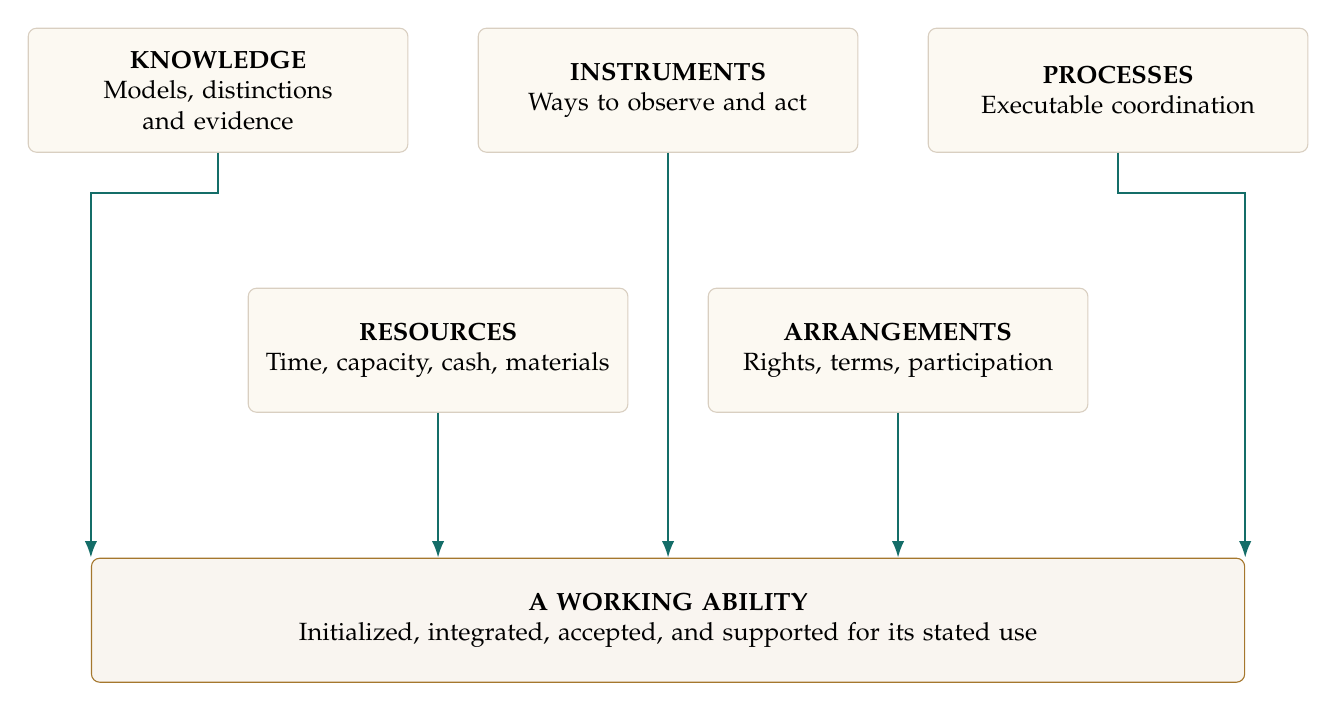
\begin{tikzpicture}[x=1in,y=1in,every node/.style={font=\small,align=center},box/.style={draw=Rule,fill=Ivory,rounded corners=3pt,text width=1.76in,minimum height=.62in,inner sep=5pt},arr/.style={-{Latex[length=2.1mm]},line width=.8pt,color=Teal}]
\node[box] (k) at (0,1.3) {\textbf{KNOWLEDGE}\\Models, distinctions\\and evidence};
\node[box] (i) at (2.25,1.3) {\textbf{INSTRUMENTS}\\Ways to observe and act};
\node[box] (p) at (4.5,1.3) {\textbf{PROCESSES}\\Executable coordination};
\node[box] (r) at (1.1,0) {\textbf{RESOURCES}\\Time, capacity, cash, materials};
\node[box] (a) at (3.4,0) {\textbf{ARRANGEMENTS}\\Rights, terms, participation};
\node[draw=Gold,fill=Gold!7,rounded corners=3pt,text width=5.6in,minimum height=.62in,inner sep=6pt] (out) at (2.25,-1.35) {\textbf{A WORKING ABILITY}\\Initialized, integrated, accepted, and supported for its stated use};
\draw[arr] (k.south)--++(0,-.2)-|(out.north west);
\draw[arr] (p.south)--++(0,-.2)-|(out.north east);
\draw[arr] (i.south)--(out.north);
\draw[arr] (r.south)--(out.north -| r.south);
\draw[arr] (a.south)--(out.north -| a.south);
\end{tikzpicture}
\caption{The components enable an outcome together. Lines mean required integration, not independent sufficient causes. A missing or incompatible element can defeat the whole.}
\end{figure}

\subsection{The witness that connects the parts}

For a starting state $x_0$, write a proposed construction witness as
\begin{equation}
w=(\pi,D,\Sigma,A,E,O).
\label{eq:witness}
\end{equation}
Here $\pi$ is the executable construction and operating policy; $D$ records dependencies and interface meanings; $\Sigma$ schedules resource use; $A$ specifies required authority and arrangements; $E$ links claims to evidence; and $O$ records continuing obligations. A policy chooses from available observations. It cannot choose a branch using a hidden environmental fact that no allowed observation reveals.

A \emph{prospective witness} says how a modeled route could work. A \emph{realized witness} additionally records the actual execution, required acceptance, and resulting obligations. A forecast of consent belongs to the former. Only a corresponding authorized action belongs to the latter.

\Needspace{6\baselineskip}
Five questions turn a parts list into a construction:
\begin{enumerate}
\item \textbf{Can it start?} Every initial prerequisite is available or reached by a feasible preceding action. Mutual promises to create each other do not start a process.
\item \textbf{Do the parts compose?} Interfaces have compatible meanings, units, versions, and operating conditions. A shared resource is not allocated twice.
\item \textbf{Can every step occur?} Time, liquidity, capacity, and authority hold at every prefix of execution, not only in the final totals.
\item \textbf{Does the intended outcome follow?} Acceptance checks the useful whole and its adverse cases, including failures shared by several components.
\item \textbf{What remains afterward?} Support, maintenance, debts, refunds, decommissioning, and retained capabilities have explicit owners and costs.
\end{enumerate}

These are substantive properties of the route. They need not become five separate committees, scores, or mandatory software modules. A small problem may be settled by one clear calculation and an executable test. A high-consequence physical system requires evidence proportionate to its consequences.

\subsection{Completeness has a boundary}

For an explicitly modeled environment $\theta$, let $\operatorname{Valid}(w;\I,x_0,\theta)$ mean that the policy's execution respects the contract, its resource prefixes, and its acceptance conditions. Robust model-relative completeness requires this for every $\theta$ in a declared set $\Theta$. A probabilistic version requires a stated reliability target under a justified distribution instead.

Neither version establishes that the modeled set contains every relevant real failure. An omitted disturbance, false interface assumption, or forged source can invalidate the conclusion. The witness must therefore distinguish a proved implication, a measured property, an assumption, and an unresolved dependency. Unknown conditions can motivate a new experiment or a construction that makes them irrelevant. They cannot become true because the narrative needs them.

The practical aim is \emph{enough justified completeness for the useful outcome}, with the residual boundary visible. Requiring omniscience would prevent action. Hiding the boundary would manufacture confidence.

\section{From available tools to a construction frontier}
\label{sec:frontier}

\subsection{A capability is an operation with conditions}

Represent the current productive state as
\begin{equation}
x=(\K,\mathcal J,\mathcal P,r,a,e,o),
\end{equation}
comprising knowledge, instruments, procedures, resources, authority/arrangements, evidence, and obligations. These categories can overlap in implementation; the notation prevents a useful file from being confused with usable equipment, accepted permission, or spendable funds.

A capability is a conditional operation: given specified inputs and a valid state, it produces an output and a changed state while consuming resources. Construction adds or changes such an operation. Requalification may remove its usable scope. Retirement may reduce obligations. A useful policy must be able to do all three.

For a declared model and horizon, define
\begin{align}
\R_{\mathrm{use}}(\I,x)&=\{y:\text{a valid policy delivers $y$ using the installed repertoire}\},\\
\R_{\mathrm{build}}(\I,x)&=\{y:\text{a valid policy delivers $y$ and may construct new means}\}.
\label{eq:frontiers}
\end{align}
The repertoire and the distinction between use and construction must be stated for the comparison. If every use-policy is also allowed in the second set, then $\R_{\mathrm{use}}\subseteq\R_{\mathrm{build}}$. The useful question is whether an accepted outcome lies in the difference under the same initial resources, authority, and horizon.

This is not evidence that an incumbent could never have built the same means. A competent comparator must receive the same construction and procurement options when the claim concerns builder quality. An example can demonstrate a limitation of an installed arrangement while a conventional constructor fully matches the proposed solution.

\subsection{Three boundaries that a build can move}

\textbf{The physical or logical boundary.} A new observation can distinguish states that old observations cannot distinguish. A new manufacturing operation can change the realizable geometry. Proof requires an appropriate model or independent physical evidence.

\textbf{The resource boundary.} The outcome was possible but not within the available money, time, energy, capacity, or risk allowance. A complete lower-cost route can make it reachable. The claim depends on the stated threshold and a fair complete alternative.

\textbf{The discovery boundary.} An adequate route was feasible, but the procedure did not find it. A better representation, search method, experiment, or construction heuristic can help. This is a gain in finding and realizing possibilities, not necessarily an enlargement of the mathematical feasible set.

The distinctions matter commercially and scientifically. A conventional solution can remove a real obstruction for a particular organization. That does not make the solution new to science. Conversely, a novel algorithm may fail to change any worthwhile outcome after integration costs.

\subsection{Complementary prerequisites and the first viable whole}

The GENESIS capability hypergraph expresses jointly necessary means \citep{boucherGenesis}. An edge $\{m_1,\ldots,m_k\}\rightarrow m'$ is useful only if there is a supported realization, a feasible resource schedule, and conditions under which it remains valid. A hypergraph can summarize the construction; labeling the edge does not construct it.

\begin{proposition}[An elementary complementarity barrier]
\label{prop:complementarity}
Suppose $|M|\ge2$, no member of $M$ is initially available, and a useful outcome has value $v>0$ only when all members are available. Each member has positive construction cost $c_i$, and no proper subset has other value in this example. A procedure restricted to single-member additions that accepts only nonnegative immediate increments builds nothing. A complete construction is beneficial when $v>\sum_{i\in M}c_i$, provided its path is feasible.
\end{proposition}

\begin{proof}
Because $|M|\ge2$, every first single-member addition leaves an incomplete set, produces no outcome value, and incurs positive cost. Starting from no members, the stated local rule therefore refuses every first addition. The complete set has net value $v-\sum_i c_i$. Feasibility is a separate condition because a positive terminal balance need not fund the earlier steps.
\end{proof}

The result is intentionally elementary. It identifies the failure of a particular local rule, not the superiority of a new planner. Ordinary joint optimization can select the same bundle. In practical construction, complementarity suggests testing a small viable whole rather than demanding that each enabling component be independently profitable.

\subsection{A loop in the diagram is not a bootstrap sequence}

A proposed factory may need a calibration instrument that it is supposed to manufacture. A calibration method may require a reference that the new process is supposed to establish. Circularity is not inherently fatal: an external seed, a temporary method, or a joint operation can start a genuine cycle. The seed and transition must appear in the witness.

\begin{proposition}[Unseeded prerequisite obstruction]
\label{prop:bootstrap}
In a discrete action model, let $U$ be a set of capabilities absent initially. If every permitted action that can create any member of $U$ requires at least one member of $U$ to be present before that action, and no exogenous event supplies one, no finite action sequence creates a member of $U$.
\end{proposition}

\begin{proof}
Assume a sequence creates a first member of $U$. Immediately before that action, no member is present, contradicting the action's required prerequisite. Equivalently, absence of every member is preserved by induction over the sequence.
\end{proof}

This result makes the first construction unusually important. It may require purchased equipment, external expertise, a coarse temporary instrument, a validated reference, or a simpler process. Access to those means must be real at the evidential level claimed. Once initialized, the cycle still needs maintenance, material and energy flows, acceptance, and replacement of its own critical dependencies.

\subsection{Building changes possibility; it need not improve it}

Let a completed build transform $x$ into $x'=T(x,w)$. The new state includes its outputs \emph{and} its consumed resources, remaining liabilities, and evidence. Comparing $\R(\I,x)$ with $\R(\I,x')$ without accounting for those changes can exaggerate progress. A machine may add useful capacity while tying up all available cash. A library may accelerate one task while making another difficult to maintain.

\begin{proposition}[Optional capability is weakly valuable under specific conditions]
\label{prop:optional}
With the same remaining resources, obligations, environment, and horizon, adding an optional operation cannot reduce optimal attainable value if every old policy remains feasible and the addition imposes no unavoidable cost. Strict improvement requires a newly feasible policy with strictly greater value.
\end{proposition}

The proof is feasible-set inclusion. Actual building usually changes resources and can create carrying costs, so the proposition does not say that every construction pays. Nor does a larger feasible set guarantee that a bounded search procedure finds a better policy. This is why \emph{learning to build} includes learning what to retire, what to buy, and what to avoid building.

\section{From a successful build to a better builder}
\label{sec:builder}

\subsection{The construction loop}

The proposed builder searches backward from a worthwhile outcome and forward from available means. Backward reasoning asks which missing conditions prevent acceptance. Forward reasoning asks what a new measurement, method, resource, or arrangement makes possible. Their intersection supplies a construction hypothesis rather than a predetermined product catalogue.

The hypothesis must name an obstruction. It can be a proved information limit, a measured capacity shortfall, an incompatible interface, an unfundable cash prefix, an unacceptable allocation of risk, or an uncertain diagnosis. Each calls for a different move. Better optimization cannot supply an absent measurement. A new sensor cannot manufacture consent. More financing cannot repair a physically invalid design.

The builder then compares direct use, acquisition, adaptation, joint construction, an informative experiment, removal of an unnecessary dependency, and non-entry. This is a set of alternatives, not a mandatory sequence. The best candidate becomes an executable witness, is challenged on consequential failures, and is tested against the original outcome. An adjudicated failure should change the construction or its diagnosis. It should not trigger a more favorable success criterion.

\begin{practicebox}
\textbf{A useful failure asks for a next construction.}\par
``The model was wrong'' is a weak lesson. ``This calibration cannot distinguish the desired signal from contact drift; obtain an independently varied reference, or change the fixture so drift no longer controls the decision'' is a construction-relevant lesson. It remains a hypothesis until its proposed remedy is tested.
\end{practicebox}

Several failures may share a cause. Repeating the same code with different prompts is not independent evidence. Conversely, a critic can be wrong. Retain a checkable counterexample or discriminating observation, adjudicate it, then repair. The loop learns from an established mechanism or a well-described uncertainty, not from the confidence of a critique.

\subsection{What should survive the build?}

A useful inheritance can have three layers:
\begin{enumerate}
\item \textbf{The working means:} a program, instrument, interface, procedure, relationship, or other usable asset.
\item \textbf{Its applicability:} the purpose it served, assumptions, evidence, failures, dependencies, rights, and conditions that invalidate reuse.
\item \textbf{Its constructor:} an executable or reproducible method for creating related means, with its own inputs, costs, and demonstrated scope.
\end{enumerate}

The third layer is often the most consequential and the easiest to overstate. A saved transcript can describe a successful build without being a reliable method for another. A general compiler can be supplied by a developer rather than learned by an agent. A method can work on a new task because the task author encoded the needed adaptation. The evidence must identify which of these occurred.

Selective retention matters. Keep the useful program, a compact mechanism, the essential evidence, and the conditions under which it should not be used. Repeated terminal logs add little when a smaller record preserves the incurred costs, failures, and lesson. Discarding redundant material is compatible with learning; deleting unfavorable results from a comparison is not.

\subsection{Four objects that can improve}

Let $z$ denote a fresh construction task, $K$ the supplied knowledge and tools, $\kappa$ a constructor, and $B$ the complete resource budget. Let $W(\kappa,z,K,B)$ report the prespecified accepted outcome together with its relevant costs and failures. When a scalar utility is appropriate, define
\begin{equation}
J(\kappa;K,B,\mathcal D)=\E_{z\sim\mathcal D}[W(\kappa,z,K,B)].
\label{eq:constructor}
\end{equation}
The task population $\mathcal D$ must be meaningful and held fixed for the claim. When benefits are incomparable, report a vector or a Pareto comparison instead of inventing a universal score.

\textbf{Artifact improvement} changes what one produced object does. \textbf{Capability inheritance} changes $K$, perhaps without changing $\kappa$. \textbf{Constructor improvement} changes $\kappa$ and is tested with matched $K$, resources, and task distribution. \textbf{Construction-learning improvement} changes a learning rule $L$ that proposes or revises constructors after development experience. It requires fresh campaigns testing the output of $L$, with development costs included.

Formally, if $h$ is development history and $\kappa'=L(\kappa,h)$, the stronger claim concerns the performance of $L$ across independently initialized development-and-confirmation campaigns. A single useful $\kappa'$ does not establish that the rule reliably produces better constructors. Searching many variants and reporting only the winner cannot estimate that reliability.

\subsection{The finished artifact must sometimes be taken away}

An especially informative transfer test removes the donor's finished artifact while preserving the candidate construction procedure. The successor requires a different output, and all arms receive equal permitted task information. If the retained procedure still improves the creation of that output, it has contributed something beyond direct artifact reuse.

This test is necessary for some claims but insufficient on its own. A conventional interpreter, compiler, engineer, or frontier agent may reconstruct the same means as well or better. An \emph{equal-content control} therefore receives the same valid specification, lessons, and construction permissions, while using an ordinary method. A further supplied-solution arm can separate finding the construction from implementing a construction already known.

The experiment in Section~\ref{sec:study} deliberately includes the donor-artifact exclusion and an equal-content control. It demonstrates the mechanics of constructing fresh programs. Because the constructor is supplied and the ordinary control ties, it does not demonstrate that experience improved the constructor.

\subsection{A better builder sometimes builds less}

A retained capability creates options and may create obligations. It can require version updates, inspection, recalibration, scarce expert attention, reserved cash, support, or decommissioning. We call these \emph{construction obligations}; the phrase is descriptive, not a new accounting category. A build is evaluated with them included.

The right decision may be to keep only a generative method, obtain a commodity service when needed, compress several overlapping tools into one simpler representation, or retire an obsolete asset. As outside methods improve, an internal construction can lose its justification. A discovery enterprise should benefit from that progress rather than preserve its own machinery for prestige.

The retained state is therefore an actively maintained means of future production. Its success is measured by what fresh work becomes feasible and worthwhile, after its costs, rather than by the size of its archive.

\section{An executable witness: constructing what the successor needs}\label{sec:study}

\begin{statusbox}
\textbf{Preserved 1.0.0 illustration.} This section carries forward the authored finite study from the published first edition \citep{learningBuildOriginal}. Its evidence remains in the original source tree. The microscopy continuation in Section~\ref{sec:continuation} is a separate empirical construction with a different protocol and acceptance boundary.
\end{statusbox}

The framework should produce something that works. We therefore accompany the
paper with a finite study that constructs new executable instruments, checks their
outputs, and asks when the complete means of using them are affordable and
available. Its purpose is to expose distinctions that a compelling diagram could
hide: a finished instrument can fail on a successor; a reusable constructor can
build a valid replacement; current rights and qualification remain necessary; and
retention can impose obligations that make the next outcome harder to reach.

\begin{statusbox}
\textbf{What is supplied and what is executed.} The task language, compiler,
specifications, alternative routes, rights scenarios, and planning costs are
authored. The generated programs and their output checks are executed. The
constructor is \emph{supplied, not learned}. No physical sensor, customer,
transaction, model call, or autonomous discovery is represented.
\end{statusbox}

\subsection{Constructing a fresh instrument}

A task specifies named integer input fields $f_j$, affine calibration coefficients
$a_j,b_j$, aggregation weights $w_j$, and a threshold $\theta$. Its required
measurement and decision are
\begin{equation}
 z(x)=\sum_{j=1}^{d}w_j\bigl(a_jx_{f_j}+b_j\bigr),
 \qquad d(x)=\mathbf 1\{z(x)\geq\theta\}.
 \label{eq:study-instrument}
\end{equation}
The compiler combines these terms into a standalone Python program. It consumes
JSON records, requires the exact integer schema, computes the measurement and
Boolean decision, and emits a specification hash. This is actual source
generation from a supplied specification, using ordinary algebra. It is not a
discovery of a new measurement law.

The source instrument computes $2a+2b+c+1$. The first successor instead requires
$2q-p+6r+1$, with different field names, coefficients, and threshold. Further
successors require four and five fields. The finished source program cannot
consume these schemas. Keeping that program alone therefore does not solve the
successors. The retained generic compiler creates three fresh programs from their
specifications; their correctness does not depend on executing the finished donor
program.

For each task we enumerate every vector in
$\{-2,-1,0,1,2\}^{d}$. A separate calculation checks both the numerical result and
the decision. A strong ordinary control directly interprets the same declarative
specification, without needing to generate a program. Table~\ref{tab:study-programs}
reports all cases. The output field named \texttt{accepted} denotes the
per-record threshold decision; commercial acceptance is not implied. Program
qualification means matching the specified result on the entire declared test
domain, including correctly negative decisions.

\begin{table}[htbp]
\centering\small
\begin{tabularx}{\linewidth}{YrrP{1.58in}}
\toprule
Task & Input cases & Both methods correct & Finished source program\\
\midrule
Source: three fields & 125 & 125 & Same task\\
Successor 1: three fields & 125 & 125 & Schema rejection\\
Successor 2: four fields & 625 & 625 & Schema rejection\\
Successor 3: five fields & 3,125 & 3,125 & Schema rejection\\
\midrule
Total & \textbf{4,000} & \textbf{4,000} & Three incompatible successors\\
\bottomrule
\end{tabularx}
\caption{Actual generated programs and the ordinary interpreter agree with the
specifications on the complete stated finite domain. These authored fresh tasks
are not independently selected natural tasks. No runtime or learning advantage is
claimed.}
\label{tab:study-programs}
\end{table}

\subsection{Completing the means of delivery}

Correct output is one component of the modeled outcome. An internal delivery
also requires a reusable testing fixture, current access terms, fresh
qualification, and production resources. An external complete service is a
separately available conventional route under its own supplied standard terms.
Missing internal consent does not disable that external alternative.

The fresh internal route costs 54 planning units and takes eight time units:
18 for construction, 10 for the fixture, 6 for current terms, 8 for qualification,
and 12 for production. Inheriting the fixture removes its repeated cost and time,
giving 44 units and six time units. Inheriting the supplied constructor additionally
changes assumed fresh construction cost from 18 to 7 and its duration from three
to one, giving 33 units and four time units. The complete external service costs
58 units and takes four time units. These are \emph{synthetic planning
assumptions}, not measured savings from compilation, labor estimates, currency, or
market quotations.

The constructor state also carries a current maintenance obligation $m$. This
must be paid even if the external service or nonentry is selected. Every delivery
expense precedes its modeled receipt of 80 units. A route is feasible only if
every cash prefix remains nonnegative, the deadline is met, and its current
rights and qualification conditions hold. Constructor acquisition and full
continuation costs are accounted for separately in the economic analysis; the
state comparison here conditions on what has already been retained.

\subsection{The frontier expands---and can contract}

Before execution, the protocol fixed cash values
$\{32,33,43,44,53,54,57,58\}$, deadlines $\{3,4,5,6,7,8\}$, two internal-consent
settings, and maintenance values $\{0,12,26\}$. Their Cartesian product contains
288 cells. Evaluating the three inherited states gives 864 complete-route
decisions. Each decision selects the least-cost feasible supplied route, or
nonentry when none qualifies. This is exact only within the declared catalogue.

\begin{table}[htbp]
\centering\small
\begin{tabularx}{\linewidth}{P{.92in}rYYY}
\toprule
Maintenance $m$ & Cells & Fresh state & Fixture-only & Constructor state\\
\midrule
0 & 96 & 12 & 22 & \textbf{40}\\
12 & 96 & 12 & \textbf{22} & 20\\
26 & 96 & 12 & \textbf{22} & 0\\
\bottomrule
\end{tabularx}
\caption{Number of cells admitting an accepted modeled delivery. The selected
grid is a finite comparison, not a probability distribution. Fresh and fixture-only
counts repeat because the maintenance obligation belongs only to the constructor
state. These unequal-state counts are not a ranking of learning algorithms.}
\label{tab:study-frontier}
\end{table}

The positive witness is transparent. With cash 33, deadline four, current internal
consent, fresh qualification, and zero maintenance, the constructor route delivers.
The fresh, fixture-only, and external routes do not fit those resources. Remove
current rights or qualification and the internal result becomes infeasible.

The adverse witness is equally consequential. With cash 58, deadline four, and
no internal consent, the fixture-only state can buy the external complete service.
Retaining a constructor with maintenance 12 leaves insufficient cash for that
same service. The additional asset has contracted the reachable set. This does
not contradict conditional state dominance: its no-greater-obligations premise
has failed. A useful retained object is not automatically a better productive
state.

\subsection{What the strong control establishes}

An ordinary analytical planner receives the same specifications, constructor
recipe, retained fixture, resource limits, rights, costs, and complete routes. It
agrees with the constructor-state planner in \textbf{all 288 decisions}. Its
ordinary interpreter also matches every generated instrument's required output.
The control is therefore not deprived of the very content responsible for the
conditional gain. Compilation is not technically necessary for these arithmetic
tasks: the interpreter already supplies the required answers. The emitted
programs demonstrate portable construction, not the uniquely necessary or
empirically cheapest implementation.

The study establishes a finite example of \emph{fresh construction using retained
means}. It does not establish that experience improved the constructor, that a
special discovery policy outperformed ordinary engineering, or that the supplied
cost advantage would occur in practice. The conventional tie is a substantive
result: productive value and proprietary methodological superiority are different
claims. The three fresh schemas demonstrate donor-artifact incompatibility; they
do not establish open-ended transfer outside the supplied language.

\subsection{Reproduction and claim boundaries}

From the versioned source package root, reproduce the preserved 1.0.0 study into a new directory:
\begin{lstlisting}
python3 -B study/study.py --output /absolute/new/replay
python3 -B study/check.py --evidence /absolute/new/replay
\end{lstlisting}
The first command generates the instruments, compact results, and all grid cells.
The second imports no producer code: it separately executes the instruments and
replays route costs and cash prefixes. This is a separate-source engineering
cross-check, not an independent institutional evaluation. The retained protocol
and result hashes bind the task definitions and implementation. Both entry
points pin the exact registered protocol; this reproduction is not a general
configurable simulator. The checker recomputes the complete reported record,
including all counts, hashes, flags, and row cardinalities. Normal and
optimized Python execution produced byte-identical reported results.

Adverse checks reject incompatible schemas, a tampered task contract, missing
current qualification, and absent internal rights, while preserving the
maintenance counterexample. Exact checking covers the authored domain and
assumptions. It does not establish real demand, observed consent, physical
qualification, measured economic productivity, or construction learning. The
next experiment must earn those stronger bridges rather than rename this witness.

\begin{thesisbox}
\textbf{The lesson.} Keeping a finished object and keeping a means of building
the next object are different achievements. Either becomes productive only when
the complete current means of accepted use are available.
\end{thesisbox}

\section{Versioned continuation: from nuclei to cell bodies}
\label{sec:continuation}

\subsection{The useful outcome and the missing means}

The beneficiary is a researcher evaluating reproducible offline image measurements. The intended ability is to run an analysis instrument, inspect the objects it predicts, obtain counts and segmentation-derived pixel areas, and determine where it meets a declared reference standard. No laboratory was recruited; these are author-defined research gates, not external laboratory or clinical certification.

The first construction concerns nucleus instances in BBBC039v1. The successor concerns whole-cell instances from the DNA and actin channels of BBBC007v1. Nucleus masks alone do not supply cell-body boundaries. The successor changes the assay, cell line, observation channels, annotation format, and required output. It therefore asks for a different instrument rather than a relabelled first run \citep{bbbc039,bbbc007}.

The initial missing means are deliberately concrete: supported data acquisition, an explicit decoder for reference annotations, an executable analysis recipe, compatible inputs and outputs, independent recomputation of acceptance, and an operating procedure. The recipe operators themselves are established morphology and watershed methods supplied by the authors. Whether that finite grammar contains a qualifying successor is an empirical question; improved ordering cannot manufacture a candidate absent from the grammar.

\begin{practicebox}
\textbf{What a usable first instrument delivers.} A researcher supplies an image within the declared input contract and receives an instance mask, object count, pixel-area records, and inspectable diagnostics. A benchmark qualification supports that contract only. Physical areas require an independently justified pixel scale; a new assay requires its own evidence and acceptance.
\end{practicebox}

\subsection{Frozen data, fields, and acceptance}

The source uses the official BBBC039v1 split: 100 training, 50 validation, and 50 test fields. The 100 training fields supply donor experience and the recipe-selection history; the 50-field validation and test sets assess the emitted source instrument. All 18 test plates also occur in training, so this is not a cross-plate transfer result. The successor uses all 16 complete BBBC007v1 fields: four lexicographically first A9 fields for calibration and twelve remaining fields for test. That structured split is not a random sample of construction tasks. One public successor assay cannot estimate general construction-learning performance.

Both datasets provide public reference annotations and state CC0 terms \citep{bbbc039,bbbc007}. The five compressed archives total 87,775,682 bytes and are identified by hashes in the acquisition and protocol records. Neither a successful download nor a matching hash establishes the scientific adequacy of the labels.

\begin{table}[htbp]
\centering\small
\begin{tabularx}{\linewidth}{@{}P{1.22in}YY@{}}
\toprule
\textbf{Contract} & \textbf{Required quality} & \textbf{Required coverage}\\
\midrule
Nucleus instrument & Mean instance F1 $\geq .70$ under matching with IoU $>0.5$; mean relative count error $\leq .20$; mean foreground Dice $\geq .85$. & Every gate holds separately on the 50 validation and 50 test fields.\\
Whole-cell successor & Mean internal-boundary F1 within 2 pixels $\geq .60$, both over all fields and over reference-boundary-bearing fields; mean count error $\leq .25$; foreground Dice $\geq .80$. & Every gate holds on both four-field calibration and twelve-field test; at least one calibration and two test fields carry reference internal boundaries.\\
\bottomrule
\end{tabularx}
\caption{Acceptance fixed in the registered research comparison. Quality in one column or cohort does not waive another requirement. Area estimates are reported as diagnostics; these gates do not establish biological area accuracy.}
\label{tab:microscopy-contracts}
\end{table}

Instance matching is one-to-one maximum-cardinality matching with IoU strictly greater than $0.5$. Relative count error is $|n_{\rm pred}-n_{\rm ref}|/\max(1,n_{\rm ref})$. The internal-boundary metric uses four-connected inner label boundaries within an eroded foreground, then symmetric precision and recall for boundary pixels within Euclidean distance two. It excludes boundaries adjacent to the background. Reporting a separate mean over fields with true internal boundaries prevents empty-boundary fields from obscuring failure on the actual separation task. Reference regions reconstructed from manual outlines remain conditional on the explicit decoder and border policy in the protocol.

The original BBBC007 boundary-focused setup permits manually outlined nuclei and foreground as inputs, following the work of Jones and colleagues \citep{bbbc007,jones2005}. Our primary contract instead requires both to be constructed from the raw channels; manual inputs appear only in the labelled diagnostic. The collection's historical one-direction boundary percentage and this protocol's symmetric F1 are also different metrics. The reported numbers therefore do not constitute a head-to-head comparison with that historical result.

\subsection{What the constructor can learn in this experiment}

Each classical constructor receives the same 24 supplied recipes, interpreter, target raw channels, four calibration references, and permitted CPU environment. Its adjustable object is the order in which those recipes are evaluated. Greedy coverage of donor performance supplies one revised order; conventional empirical ranking over exactly the same donor table supplies the primary matched comparison. This is an update to a parameter of a supplied finite constructor. It is not discovery of the recipe operators or an autonomous revision of the construction language.

\begin{table}[htbp]
\centering\small
\begin{tabularx}{\linewidth}{@{}P{1.55in}Y@{}}
\toprule
\textbf{Arm} & \textbf{Method and retained means}\\
\midrule
Fixed, no history & A frozen expert-informed order; no donor history or privileged donor recipe.\\
Ordinary reuse & Execute the donor recipe first, then the fixed order without duplicates.\\
Updated, no artifact & Donor-derived greedy-coverage ordering, without privileged donor-artifact execution.\\
Updated with artifact & Execute the donor recipe first, then the greedy order without duplicates.\\
Same-content empirical & Conventional ranking by aggregate donor quality, with the full identical donor table.\\
Full enumeration & Execute all 24 recipes and select with the same calibration quality ordering.\\
\bottomrule
\end{tabularx}
\caption{Six separately executed arms. ``No artifact'' removes privileged donor placement, not the corresponding recipe from the shared bank. The primary contrast is greedy coverage versus same-content empirical ranking.}
\label{tab:six-arms}
\end{table}

Ranked arms stop only at the first candidate satisfying every calibration gate. Each may execute all 24 candidates; a restricted search budget is not used to manufacture an advantage. If none qualifies, the best calibration candidate is retained and labelled unqualified. Full enumeration always evaluates the complete bank. Target scores are not shared across arms. Each selected instrument and its order are sealed before its test stage.

The primary work endpoint is a candidate execution across all four calibration fields. A local advantage requires accepted held-out functionality and a strict reduction in those executions against the same-content empirical arm, without loss of acceptance. CPU time, wall time, checking, donor acquisition, maintenance, and total lineage costs are separate outcomes. Faster prefix search alone cannot establish an overall advantage. The present reproduction uses already exposed data and outcomes; it measures reproducibility rather than producing a new hidden confirmation sample.

\subsection{The practical specialist alternative}

A separately registered CellposeDINO \texttt{cpdino-vitb} route supplies a strong existing specialist. The fixed implementation uses Cellpose 4.2.1.1, pinned DINOv3 source, and a pinned 343,599,997-byte model. It runs on CPU with the frozen inference configuration, without fine-tuning or calibration-based parameter selection. Manual references are excluded from predictor inputs. The upstream documentation identifies this model as the smaller DINOv3-ViT-B member of the CellposeDINO family \citep{cellposeModels}.

The extra pretrained stock is part of the explanation and the cost boundary. Its operation must not be credited to local donor experience or folded into the matched six-arm comparison. Pretraining overlap with the evaluation images is unknown. The code, weights, training-data terms, and DINOv3 terms are distinct rights questions; the recorded scope is research operation, with no established commercial entitlement and no redistribution of upstream source or weights. A working specialist route can be adopted without claiming that it is a newly invented algorithm or an exclusively enabled successor.

\subsection{Preserved failures and representation amendments}

The published preregistration lineage records two failed constructions before target test prediction or scoring. The first encountered Boolean outline storage that violated an integer-only loader assumption. A lossless Boolean-to-integer conversion was registered as a narrow repair. The second encountered RGB raw TIFFs while the observation contract required scalar channels. Its calibration had already exhausted all 24 recipes in every arm, selecting the same unqualified recipe.

The next amendment introduced one common, supplied RGB-to-L convention from Pillow 13, while leaving scalar arrays unchanged. This conversion is generally lossy. It does not recover physical fluorescence or justify a radiometric claim; it changes the represented observation contract explicitly. It applies to raw DNA and actin only, preserves spatial geometry and field membership, and uses the same convention for the classical and specialist routes. The frozen review checked all $2^{24}$ RGB triples against independent fixed-point arithmetic, with a shared Pillow dependency. That is an implementation check, not scientific calibration or external certification.

The specialist preparation also required a narrowly recorded state-loading exception for two nonlearned diameter scalars; trained tensors remained subject to the declared audit. These failures identify integration assumptions, not an opportunity to lower acceptance thresholds. The historical sources and compact review records survive at their published commits. The appendix distinguishes those records from the artifacts produced by the new reproduction and from historical costs that cannot be reconstructed.

\subsection{Results and decision}
\subsubsection{Classical nucleus instrument: the complete source gate fails}

All 24 recipes were evaluated on the 100 donor fields, for 2,400 recipe--field executions. The registered donor selection chose \texttt{r17}. Its training mean count error was 0.591295, so the selected donor was already unqualified on training. The protocol requires continuing the successor comparison even after that failure; it does not permit claiming that an accepted donor enabled an accepted successor.

On the official source cohorts, \texttt{r17} passes every test-set gate but fails the validation count-error gate. Complete source qualification requires both cohorts, so the emitted classical nucleus instrument is \textbf{unqualified}. Its operability and strong performance on some endpoints do not waive the failed requirement.

\begin{table}[htbp]
\centering\small
\begin{tabularx}{\linewidth}{@{}P{1.2in}rrrrY@{}}
\toprule
\textbf{Cohort} & \textbf{Fields} & \textbf{Instance F1} & \textbf{Dice} & \textbf{Count error} & \textbf{Gate verdict}\\
\midrule
Validation & 50 & 0.884357 & 0.910637 & 0.216173 & Fail count error\\
Test & 50 & 0.897397 & 0.931317 & 0.088311 & Pass all three\\
\midrule
Required & & $\geq .70$ & $\geq .85$ & $\leq .20$ & Both cohorts\\
\bottomrule
\end{tabularx}
\caption{Classical source recipe \texttt{r17}. Values are means over fields, rounded to six decimal places; count error is the mean of per-field relative errors, not an error computed from pooled counts. Exact values remain in the machine-readable results.}
\label{tab:classical-source}
\end{table}

\subsubsection{Whole-cell construction: failure and a matched comparison tie}

Every successor arm executed all 24 recipes, or 96 calibration recipe--field evaluations per arm. No candidate met every calibration gate. All six arms selected \texttt{r12} by the same registered fallback ranking and then failed the test boundary requirement. Each of the four calibration and twelve test fields has reference internal boundaries; the all-field and boundary-bearing-field F1 means are therefore equal here. Favorable foreground overlap and count error do not substitute for the missing boundaries.

\begin{table}[htbp]
\centering\small
\begin{tabularx}{\linewidth}{@{}P{1.12in}rrrrY@{}}
\toprule
\textbf{Cohort} & \textbf{Fields} & \textbf{Boundary F1} & \textbf{Dice} & \textbf{Count error} & \textbf{Gate verdict}\\
\midrule
Calibration & 4 & 0.250398 & 0.850357 & 0.086298 & Fail boundary\\
Test & 12 & 0.309897 & 0.861007 & 0.104715 & Fail boundary\\
\midrule
Required & & $\geq .60$ & $\geq .80$ & $\leq .25$ & Both cohorts\\
\bottomrule
\end{tabularx}
\caption{The same selected whole-cell recipe \texttt{r12} and scores in all six classical arms. Each arm separately evaluates its calibration candidates and selected test instrument. All 16 successor fields are boundary-bearing.}
\label{tab:classical-successor}
\end{table}

The primary greedy-coverage versus same-content empirical contrast saves \textbf{zero candidate executions}; both search all 24 and produce the same unqualified selected instrument. There is no local accepted construction advantage and no established lifecycle advantage. This is an observed tie in selected instrument, quality, and candidate count on this comparison. Runtime measurements can differ; the result is not a statistical equivalence claim over a population of construction tasks.

The full-enumeration control also exhausts the bank and fails. Thus the result is not caused by denying a conventional method sufficient search. Under these fixed operators, observations, calibration fields, and gates, another ordering alone cannot produce an accepted candidate. This conclusion applies to the tested bank, not to all methods for cell segmentation.

\paragraph{A controlled explanation of convergence.}
The six arms are deterministic policies over one supplied grammar, not six separately prompted language models. Their original executions contain four distinct proposed orders. All 96 recipe--calibration-field records per arm agree in prediction hashes and scientific metrics when aligned by recipe and field. A separately frozen diagnostic called the unchanged constructor with 33 order/settings interventions, comprising 30 unique orders. It replaced only the expensive evaluator boundary with an explicitly labelled adapter returning the retained calibration scores. Every replay exhausted 24 candidates and selected \texttt{r12}; there were 792 cached evaluator calls and no new image inference in this part. The highest calibration boundary F1 in the whole bank was 0.250398. The observed convergence is explained by shared candidate failure and the common fallback ranking, not identical ordering or independent model agreement. This is a mechanism check on exposed records, not a fresh task or evidence of improved construction learning.

\subsubsection{Diagnostics: what the failure does and does not localize}

The unchanged donor artifact, applied as a labelled diagnostic on the twelve successor test fields, obtains boundary F1 0.072995 and foreground Dice 0.537565 and is unqualified. The separate oracle-input diagnostic supplies manual nuclei and manual foreground to \texttt{r12}; its test boundary F1 is 0.671256, Dice 0.999933, and count error 0.159935. It meets the numerical test gates only with privileged reference-derived inputs, so it is \textbf{not a qualified raw-channel instrument} and not a primary arm.

The diagnostic supports investigating how reliable seed nuclei and foreground can be constructed from permitted observations. Because both inputs change together, it does not isolate which one is decisive, demonstrate a practical way to obtain them, or establish success on a new cohort. A new boundary method is one possible next construction; better construction of its input means is another. The reference-assisted result must not be presented as an ordinary deployment option.

\paragraph{Separating the two input interventions.}
A new diagnostic froze \texttt{r12}, the unchanged acceptance criteria and the four already exposed calibration fields before executing a $2\times2$ component comparison. No target test pixels were decoded. Each condition called the existing segmentation code and was scored by both the producer's metric code and the separately implemented checker. The baseline matched all archived calibration prediction hashes and scores. The combined intervention matched a new call to the unchanged producer's oracle path on these same four fields; no prior combined-reference calibration output was claimed.

\begin{table}[htbp]
\centering\small
\begin{tabularx}{\linewidth}{@{}YrrrP{.78in}@{}}
\toprule
\textbf{Calibration inputs} & \textbf{Boundary F1} & \textbf{Dice} & \textbf{Count error} & \textbf{Numerical gate}\\
\midrule
Raw seeds, raw foreground & 0.250398 & 0.850357 & 0.086298 & Fail\\
Reference seeds, raw foreground & 0.195353 & 0.829797 & 0.111399 & Fail\\
Raw seeds, reference foreground & 0.615828 & 0.999903 & 0.090194 & Pass\\
Reference seeds and foreground & 0.714909 & 0.999903 & 0.165064 & Pass\\
\bottomrule
\end{tabularx}
\caption{Fixed-recipe interventions on four exposed calibration fields. A numerical pass with reference foreground does not qualify a raw-input instrument or imply that every individual field passes. All sixteen component masks received separate-code rescoring; eight additional producer-control segmentations were charged.}
\label{tab:component-diagnostic}
\end{table}

Foreground replacement alone increased mean boundary F1 by 0.365430, whereas seed replacement alone decreased it by 0.055045. This favors investigating foreground recovery before a seeds-only repair in this implementation. The raw-foreground branch unions its mask with the supplied seeds, so changing seeds can also affect foreground; these are software-branch interventions, not isolated biological causal effects. Nearly perfect Dice with reference foreground is expected from the privileged input. The complete registration, code, masks, controls and replay checks are in \texttt{construction/diagnostics/}. Neither diagnostic supplies untouched confirmation cases or changes the original failure verdicts.

\paragraph{Constructing and rejecting one practical repair.}
The diagnostic led to one separately frozen, assistant-authored ordinary composition: take the union of the pinned specialist's final whole-cell instances as a foreground proposal, then apply the unchanged \texttt{r12} DNA-seeded watershed. The actual composition was executed on the four saved specialist calibration predictions, whose original raw-input inference and identities are retained. No reference foreground or nuclei were supplied to this candidate. Its mean boundary F1 was 0.296809, Dice 0.861057, and count error 0.081112. It improved the classical boundary endpoint but remained below the fixed specialist's 0.386561 and failed the unchanged 0.60 criterion.

The frozen stop rule was enforced: zero target test fields were scored, no parameter was tuned, and no new neural inference was performed for this failed candidate. The reusable raw-input command is included, but full fresh execution of that command is not claimed. The observed result is a failed composition from identified, previously executed constituent outputs. Its 3.263 CPU seconds and 1.755 wall seconds are additional work. The original four specialist fields already incurred 122.037 CPU seconds in segmentation (122.637 CPU and 122.650 wall seconds at the enclosing field boundary); these constituent costs are attributed, not charged a second time. The registration, implementation, masks, adverse outcome and stop receipt are in \texttt{construction/repair/}. Reliable foreground remains an unmet requirement; this available substitution did not construct it.

\subsubsection{Pretrained specialist: a qualified first route, a failed successor}

The fixed CellposeDINO route meets every nucleus gate on both official 50-field cohorts. Its test instance F1 is 0.949103, foreground Dice 0.967232, and mean relative count error 0.070837. It is therefore \textbf{qualified for the declared source research contract}. The practical construction consists of integrating and operating the pinned existing specialist with the input adapter, reference interpretation, measurements, and checks. It does not establish that the local constructor learned the specialist's competence or that pixel-area estimates are validated biological measurements.

The same specialist fails the whole-cell boundary gate on both calibration and test. Its test boundary F1 is 0.505568, below the required 0.60, despite passing the foreground and count gates. All 16 successor fields carry reference internal boundaries, so the boundary-bearing-field mean also fails. The successor is \textbf{unqualified}.

\begin{table}[htbp]
\centering\small
\begin{tabularx}{\linewidth}{@{}P{1.52in}rrrrY@{}}
\toprule
\textbf{Cohort} & \textbf{Fields} & \textbf{Primary F1} & \textbf{Dice} & \textbf{Count error} & \textbf{Gate verdict}\\
\midrule
Nuclei: validation & 50 & 0.953878 & 0.967388 & 0.066573 & Pass all three\\
Nuclei: test & 50 & 0.949103 & 0.967232 & 0.070837 & Pass all three\\
Cells: calibration & 4 & 0.386561 & 0.860566 & 0.130928 & Fail boundary\\
Cells: test & 12 & 0.505568 & 0.886682 & 0.200904 & Fail boundary\\
\bottomrule
\end{tabularx}
\caption{The fixed pretrained specialist on all 116 registered fields. Primary F1 means instance F1 for nuclei and internal-boundary F1 for cells; the different gates are given in Table~\ref{tab:microscopy-contracts}. Entries are field means rounded to six decimals. The source qualifies only because both nucleus cohorts pass; the successor requires both whole-cell cohorts and fails.}
\label{tab:specialist-results}
\end{table}

On this successor test cohort, the specialist achieves higher boundary F1 than the selected classical recipe, but also has higher count error; neither meets the complete contract. Its additional pretrained stock is a distinct resource, not the product of the local ordering update. The specialist was chosen after classical source outcomes and registered before its own inference. Potential pretraining overlap with these public images is unknown. These are findings from an exposed reproduction, not evidence of unseen-data generalization or a newly concealed comparison. Figure~\ref{fig:microscopy-examples} shows two fields chosen by declared test order, without using their scores; the complete cohorts determine the verdicts.

\subsubsection{Measured work and its boundary}

The completed classical run records 696.935 CPU seconds and 696.703 wall seconds across donor construction, source evaluation, and successor construction/evaluation, including the two labelled diagnostics. The separate completed 116-field specialist session records 4,969.507 CPU seconds and 4,970.035 wall seconds. These are measured stage or session boundaries from this reproduction. They exclude dependency setup, data acquisition, independent verification, authoring, upstream pretraining, unavailable earlier execution costs, and economic costs. They are not a whole-lineage total or a monetary price. The full report retains per-arm times alongside candidate counts so an endpoint tie is not misrepresented as identical timing.

The classical ledger records three completed attempts and no interrupted or orphaned attempt. Its negative interruption flag describes that recorded state, not verified absence of unrecorded work. The origin of 138 byte-identical residual files remains unresolved: they could be copies or products of additional execution. Any associated extra work and cost are therefore unknown. The projection preserves the measured charges and does not establish that all classical execution or cost has been captured.

The new order/component diagnostic adds 8.465 CPU seconds and 7.058 wall seconds, including its 24 actual segmentations and separate-code scoring; the order interventions themselves use cached scores. Its reproduction adds a separately recorded 8.896 CPU seconds and 7.278 wall seconds. These costs are outside the original classical stage total. The qualification packet separately preserves the installer failure, repair tests and real candidate-package inference. Nested operation and wrapper timings must not be counted twice; total authoring, human effort and monetary billing remain unknown.


\subsection{What the continuation can establish}

A qualifying first instrument establishes a bounded computational capability on the recorded data and input contract. A successor failure localizes a remaining requirement; it must remain a failure even when foreground or count diagnostics look favorable. A tie against same-content empirical ranking supplies no evidence of a better constructor. Failure to qualify from a finite recipe bank does not prove that no segmentation method can qualify.

The observed classical failure directs the next experiment toward the means of producing adequate boundaries, including reliable seed nuclei and foreground. The rational next experiment therefore follows the diagnosed missing means. If the bank is exhausted, another ordering of the same bank has no acceptance gain to discover. A boundary-specific representation, observation, algorithm, or licensed specialist is a candidate next construction. It must be frozen and compared on a new confirmation cohort, with strong complete alternatives and the costs of acquiring that capability. The current result motivates that question; it does not answer it by proposing the remedy.


\begin{figure}[htbp]
\centering
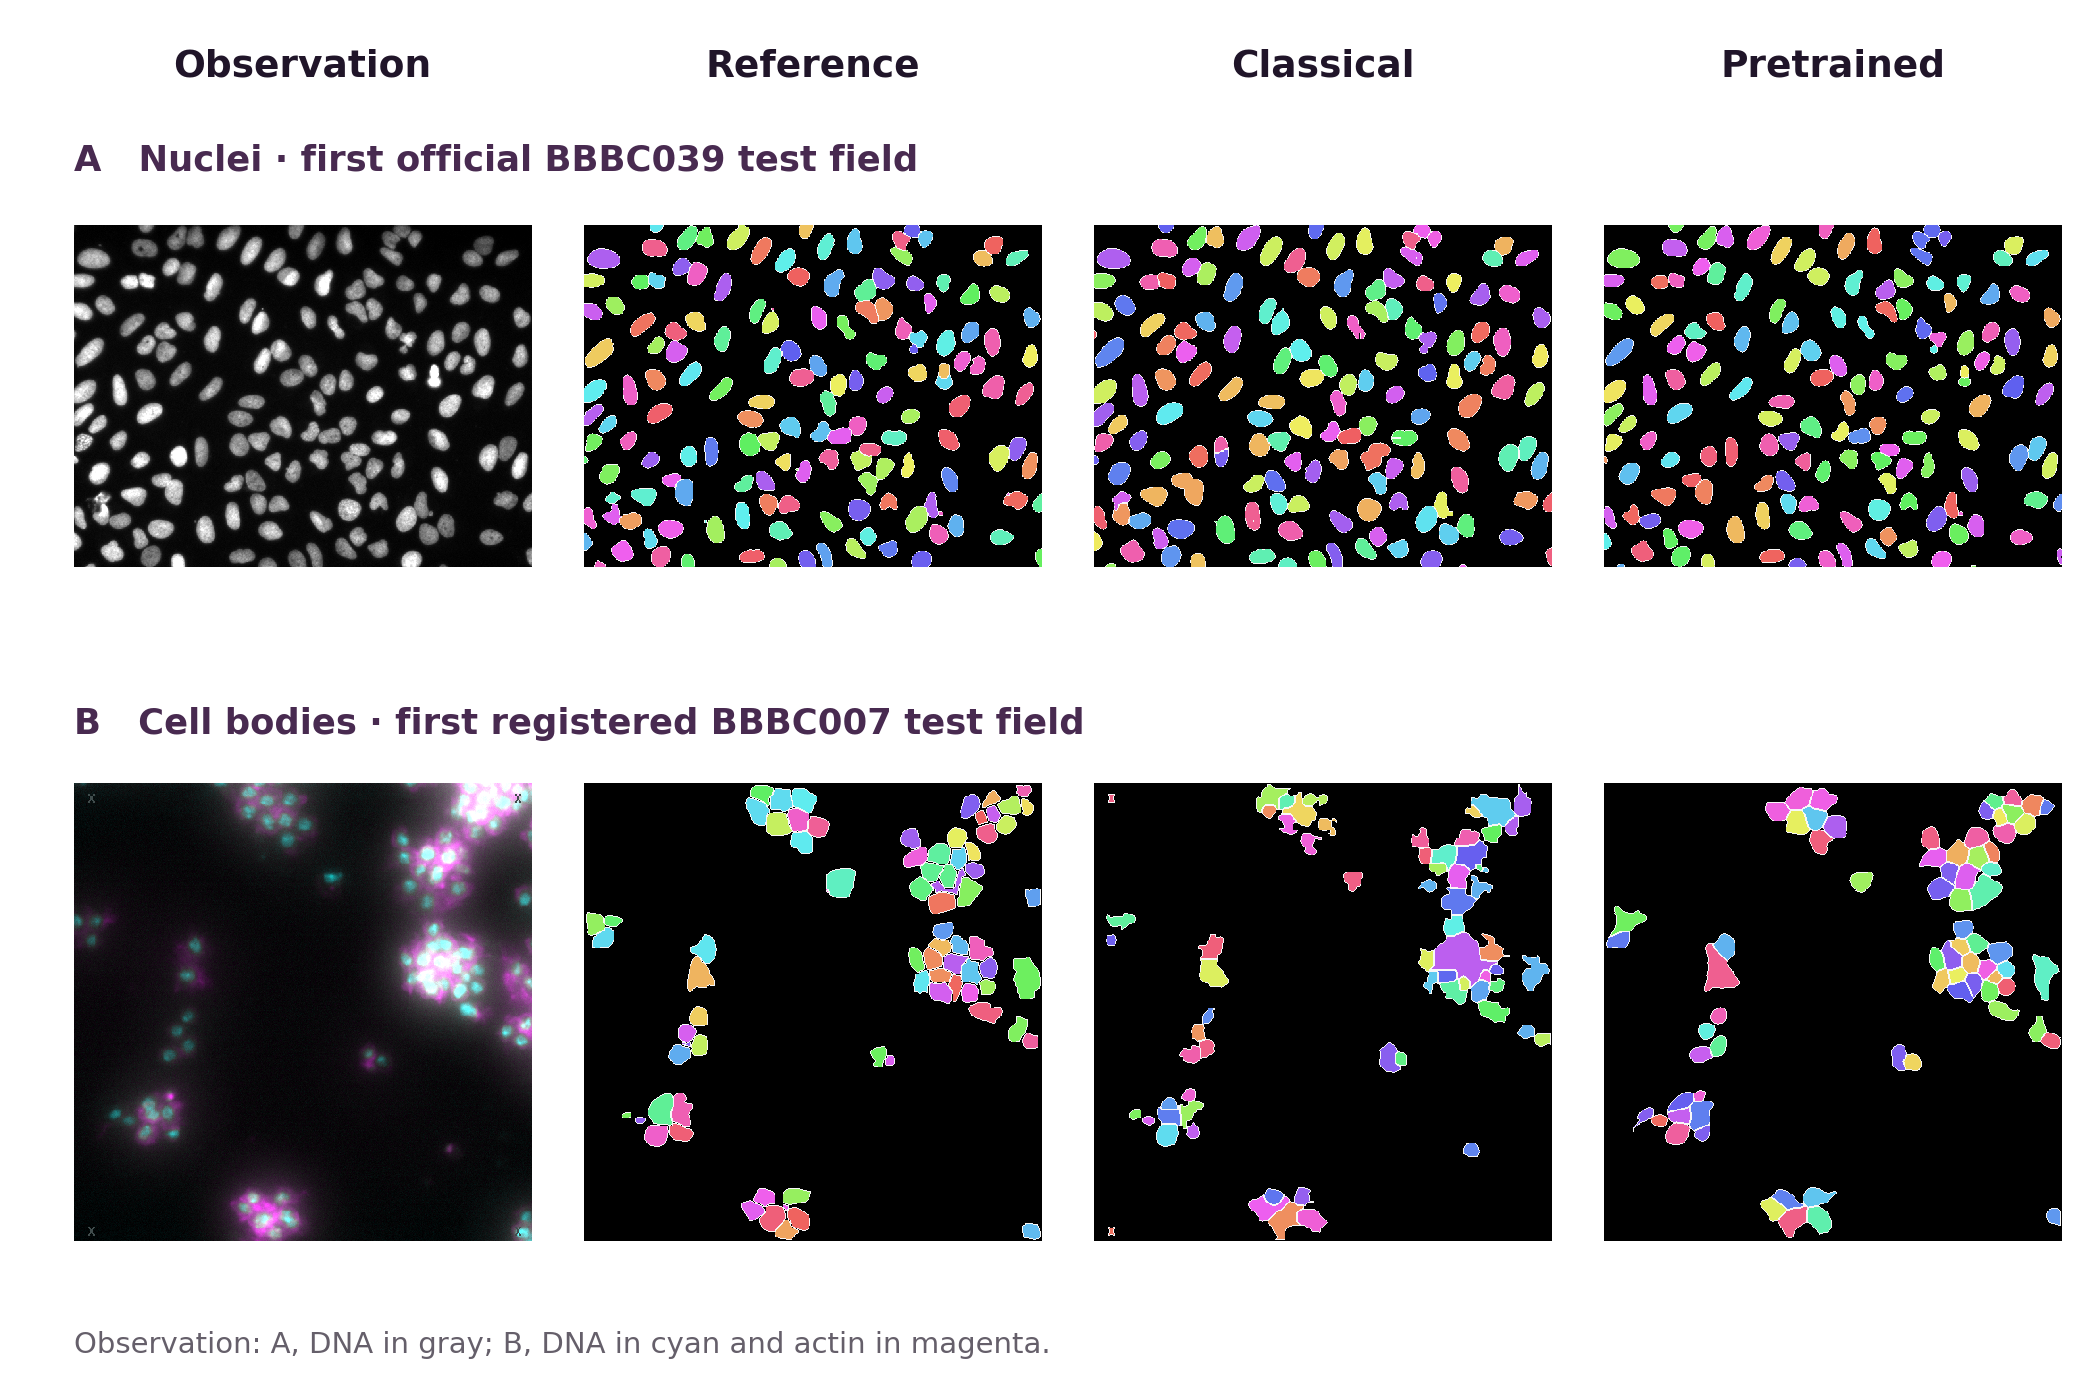
\includegraphics[width=\linewidth]{construction/figures/protocol-first-fields.png}
\caption{Two test fields selected by declared order, without using their scores: the first official BBBC039 test field and the first registered BBBC007 test field. Columns show the canonical observation, registered decoded reference, classical prediction (\texttt{r17} for nuclei; \texttt{r12} for cells), and fixed pretrained prediction. Full fields are shown without cropping. Each observation channel uses linear clipping at its first and ninety-ninth percentiles \emph{for display only}; inference and scoring inputs are unchanged. Colors distinguish instances within a panel and do not imply correspondence across panels. White inner edges aid visibility. The BBBC007 masks retain the registered complete-in-frame convention. These examples illustrate outputs; they do not replace the cohort results. Exact field identities, input and mask hashes, display ranges, and rendering source are retained in the accompanying figure receipt.}
\label{fig:microscopy-examples}
\end{figure}
\FloatBarrier

\section{Buildability includes the means of paying for the build}
\label{sec:economy}

\subsection{The arrangement can be the missing instrument}

A technically feasible construction may remain unused because its beneficiaries are fragmented, its risks are misallocated, or its funding arrives too late. A shared testing facility, a staged acceptance contract, compatible access rights, or a division of responsibilities can be part of the complete means. Such arrangements are construction hypotheses, not inferred agreements.

For participant $i$, a proposed arrangement should compare its expected utility $U_i$ with an explicit outside option $U_i^{\mathrm{out}}$. Modeled voluntary participation requires
\begin{equation}
U_i\ge U_i^{\mathrm{out}}\qquad\text{for each required participant }i.
\label{eq:participation}
\end{equation}
This condition is neither observed consent nor a proof of truthful behavior or coalition stability. It depends on supplied beliefs, information, alternatives, and enforceability. Real acceptance must be obtained at the appropriate stage. New technology can improve competitors' outside options as well as the proposed builder's costs.

\emph{Invent the Economy} makes this joint search explicit \citep{boucherEconomy}. A component with poor stand-alone returns can belong to a worthwhile package. Conversely, positive combined surplus may fail to support acceptable individual terms. The construction brief should identify who benefits, who contributes, when each acts, what each can refuse, and which complete alternative each could choose.

\subsection{Every cash prefix must be feasible}

For a declared cash schedule, write cumulative paid construction and operating costs as $C(t)$, cleared receipts as $R(t)$, received external financing as $F(t)$, financing repayments and distributions as $D(t)$, and required protected funds as $Q(t)$. With opening cash $b$, available cash is
\begin{equation}
A(t)=b+R(t)+F(t)-C(t)-D(t)-Q(t).
\label{eq:cash}
\end{equation}
The route requires $A(t)\ge0$ at every event time. $Q(t)$ must exclude amounts already counted as paid costs or repayments; releases from protection reduce $Q$ rather than create revenue. The equation is a cash-feasibility statement, not a replacement for an operating ledger or an accounting standard.

For a fixed schedule without new financing, the minimum opening cash implied by these events is
\begin{equation}
b_{\min}=\max\left\{0,\sup_{t\le T}\big[C(t)+D(t)+Q(t)-R(t)\big]\right\}.
\label{eq:prefunding}
\end{equation}
A positive terminal contribution does not remove an earlier funding shortfall. A promised investment is not received financing. Refund exposure, supplier commitments, and support obligations can remain after collection. A lower complete cost is useful only when the revised sequence can actually occur.

Starting capital is a design variable for a new economic comparison. Small staged construction, outside financing, a larger initial facility, and non-entry may all be legitimate alternatives. Their terms, costs, downside, and timing belong in the comparison. An earlier fixed-capital experiment retains its original assumptions; it is not silently topped up to make a new result attractive.

\subsection{What the finite study says about continuation}

The study uses synthetic planning units, with no currency interpretation. Its source route costs 54 and produces an assumed receipt of 80 after accepted delivery. Preserving the fixture alone leaves a successor cost of 44. Acquiring the supplied reusable constructor costs 9; each successor then costs $33+m$, where $m$ is its current maintenance obligation. Thus, for $n$ successors,
\begin{align}
C_{\mathrm{fixture}}(n)&=54+44n,\\
C_{\mathrm{constructor}}(n,m)&=54+9+n(33+m),\\
\Delta C(n,m)&=n(11-m)-9.
\label{eq:retention}
\end{align}
Constructor retention is strictly cheaper exactly when $n(11-m)>9$, conditional on the same acceptance, valid current rights, deadlines, fixture availability, and feasible cash prefixes. At $m=0$, three successors save 24 units after acquisition. At $m=12$, every additional successor makes this cost comparison worse. The parameters illustrate a threshold; they are not observed market costs or evidence of increasing returns in a real enterprise.

The distinction between \emph{later}, \emph{financed by}, and \emph{enabled by} is visible even here. An illustrative cash path starting at 54 spends the source cost, collects the modeled 80, pays 9 for acquisition, and can prepay the next 33-unit delivery. Yet the source's net contribution is only 26. If all opening capital must remain protected, the 26 does not cover acquisition plus the next 33. The path is feasible using available modeled cash; it is not, on that rule, fully funded by unrestricted earnings alone.

Likewise, a retained constructor can make a 33-unit successor affordable where a 44-unit fixture-only route is not. To establish this as a \emph{causal resource advantage}, compare equally resourced successors that may build or buy alternative means. To establish the value of acquiring the constructor, charge its acquisition and prior failed development as well. State-level reachability and whole-lineage investment value answer different questions.

\subsection{Value creation and value capture must remain connected}

An enterprise can use accepted value to sustain future construction through prices, subscriptions, licensing, shared facilities, or other voluntary arrangements. The form should reward the useful outcome and bear the necessary obligations. Billing unnecessary operations can conflict with an intelligence whose best contribution is to eliminate those operations.

Complete economic cost includes search, unsuccessful candidates, development, acquisition, production, checking, integration, maintenance, support, financing, and residual liabilities. The costing policy should explain amortization and allocation without counting one expense twice or crediting the same receipt to several generations. Included assistant resources do not imply zero underlying economic cost; unavailable bills remain unknown.

Commercial recurrence need not prove scientific novelty. A known method can support an excellent business. Scientific construction need not immediately produce a sale. The desired flywheel joins useful capability, voluntary accepted delivery, resources available for continuation, and a tested successor contribution; each connection retains its own evidence.

\section{How to establish that intelligence learned to build}
\label{sec:evaluation}

\subsection{A prospective campaign, not a gallery of successes}

The empirical target is a sequence of consequential construction tasks whose acceptance is defined before results are observed. Development tasks may reveal useful mechanisms. Confirmation tasks must require fresh outputs, come from an independently motivated population, and be protected from repeated adaptation. Many inputs to one generated program are correctness cases, not independent inventions.

A practical campaign begins with a valuable outcome that current complete alternatives do not adequately serve under a stated constraint. Compare at least three materially different possibilities when selecting a new flagship, rather than several cosmetic variations of a convenient benchmark. Selection evidence should explain the potential consequence and the decisive first construction, including why the strongest available complete alternative leaves a residual.

The selected campaign records every registered attempt, complete resource use, accepted outcomes, and compact failure lessons. It permits negative results, ordinary winners, justified refusal, and retirement. It does not restart the same failed comparison under a new title until a favorable result appears.

\subsection{Cross the method with the means}

At fixed underlying model, information access, and budget, cross the old and new constructors with the old and new capability stock:
\begin{table}[htbp]
\centering\small
\begin{tabularx}{\linewidth}{@{}P{1.35in}YY@{}}
\toprule
 & \textbf{Original means $K_0$} & \textbf{Retained means $K_1$}\\
\midrule
Original constructor $\kappa_0$ & Baseline construction. & Effect of additional content and tools under the old method.\\
Revised constructor $\kappa_1$ & Procedure effect without the new asset stock. & Joint effect and interaction between procedure and stock.\\
\bottomrule
\end{tabularx}
\caption{A causal comparison structure, not a claim that the four cells have been measured in this edition. Starting costs and obligations must be aligned for the intended estimand.}
\label{tab:factorial}
\end{table}

For a common held-out population, define the procedure effect at fixed means as
\begin{equation}
\Delta_{\kappa}(K_j)=J(\kappa_1;K_j,B,\mathcal D)-J(\kappa_0;K_j,B,\mathcal D).
\end{equation}
The interaction is the difference between these effects at $K_1$ and $K_0$. A revised method may be useful only with the representation it helped create. That is a joint mechanism, not a reason to hide the other cells. Cross underlying model versions as well when attributing gains to institutional learning rather than external model progress.

There are two valid resource questions. A \emph{current-state} test asks what can be built now from a specified inherited state. A \emph{lineage} test asks whether acquiring and maintaining that state improved total results. The latter charges development, failed search, migration, and maintenance to the appropriate arms. Neither should quietly answer the other's question.

\subsection{Controls that make the claim interpretable}

\textbf{Artifact exclusion.} Withhold the donor's finished output; require a genuinely different successor. Retain the proposed construction method and its legitimate information.

\textbf{Equal-content ordinary reuse.} Supply the same specification, lessons, data, and means to a competent conventional method. This tests whether the proposed procedure adds value beyond saved content.

\textbf{Strong unrestricted construction.} Allow a capable specialist, frontier agent, or engineer the same construction, procurement, coordination, and financing permissions. A control restricted to old tools cannot establish superiority over the best complete route.

\textbf{Supplied-solution realization.} Give each arm a correct construction description. If the advantage disappears, the difference concerned finding the construction; if it persists, investigate implementation, integration, or verification rather than calling everything discovery.

\textbf{Dependency and obligation perturbations.} Change interfaces, revoke only the permissions actually being varied, invalidate calibration, remove the fixture, introduce capacity conflicts, and test maintenance. Retained capability is conditional on these facts.

\textbf{Negative opportunities.} Include cases where the old method is already adequate, construction does not pay, or no valid route is found. Measure missed useful opportunities and invalid promotions as well as accepted successes.

These controls can be selected for a narrower registered claim; every project need not run every possible arm. Omitted controls limit attribution. They do not justify silently asserting the stronger conclusion.

\subsection{Measure outcomes, not the appearance of activity}

The primary engineering outcomes are acceptance, complete cost and time to acceptance, resource feasibility, and the scope of the constructed capability. Record interventions, corrections, failures, support burden, and whether the successor depends on retained means. Report distributions or paired outcomes when there are independent tasks, with uncertainty appropriate to the sampling and stopping scheme.

When measuring productivity, distinguish a competent frontier-AI operation from competent human workers using conventional software under the same useful outcome. Count actual or explicitly modeled human intervention inside the AI operation. Preserve ordinary software's genuine automation in the human comparator. Human-plus-AI providers, other autonomous providers, and self-service are additional commercial alternatives. None may be weakened to manufacture a result.

A learned quality estimate cannot substitute for the actual acceptance boundary. Multiple AI reviewers can share a blind spot. A separately implemented checker is useful procedural separation, not an external institutional audit. Natural scientific and industrial tasks need independent measurements, domain-valid uncertainty, and evidence about the observations the evaluation itself might miss.

\subsection{From the current instrument to a decisive next campaign}

The microscopy continuation tests a narrow part of the larger application, a \emph{construction assistant for scientific instruments}: given an authorized measurement purpose, produce a usable acquisition or analysis instrument, its interfaces and calibration procedure, and evidence that it supports the intended decision. The product hypothesis is an ability the user can operate and maintain, not a transcript of agents discussing a build.

An initial physical campaign could ask whether a new observation or fixture separates an internal sample property from contact effects that defeat the installed setup. The first test must compare strong existing inverse methods, uncertainty analysis, and equally permitted engineering. If an existing complete route already answers the question, adopt it and revise the alleged missing means. A simulator cannot validate an observation never acquired.

After the first qualified construction, freeze the retained method before revealing a different measurement objective. Compare fresh construction with and without the method, including an equal-content conventional route and all adaptation costs. Only then test a voluntary delivery arrangement. This sequence addresses a consequential dependency of the GENESIS programme without treating the present paper as a completed instrument business.

\section{The horizon: build the means of further construction}
\label{sec:horizon}

\subsection{Scientific instruments are a particularly valuable beginning}

A new instrument can change which questions are answerable. A better experiment can change which design uncertainties remain binding. A production process can then turn that knowledge into repeatable material capability. This gives a construction a second possible consequence: it may improve the means of discovering and realizing another construction.

The relationship is causal only when the successor actually depends on the new means relative to strong alternatives. A later project that uses the same codebase is not enough. Neither is a story that every useful invention somehow contributes to everything after it. Identify the specific observation, operation, representation, resource, or arrangement the predecessor supplied; remove or replace it in a fair comparison; measure the successor consequence.

Three ambitious candidate families illustrate different mechanisms. A new \emph{measurement operation} can expose an otherwise unidentifiable property. A new \emph{conversion or manufacturing process} can turn an unusable input into a qualified component. A new \emph{productive arrangement} can make complementary facilities, demand, expertise, and funding viable together. These are research directions, not completed products of this edition.

\begin{figure}[htbp]
\centering
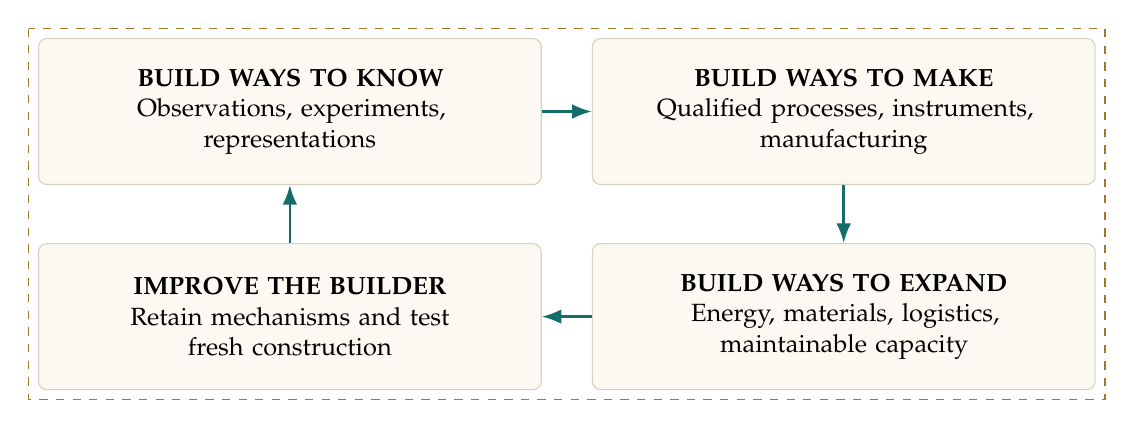
\begin{tikzpicture}[every node/.style={font=\small,align=center},node distance=.29in and .25in,box/.style={draw=Rule,fill=Ivory,rounded corners=3pt,text width=2.32in,minimum height=.73in,inner sep=7pt},arr/.style={-{Latex[length=2.5mm]},line width=.9pt,color=Teal}]
\node[box] (observe) {\textbf{BUILD WAYS TO KNOW}\\Observations, experiments,\\representations};
\node[box,right=of observe] (produce) {\textbf{BUILD WAYS TO MAKE}\\Qualified processes, instruments,\\manufacturing};
\node[box,below=of produce] (expand) {\textbf{BUILD WAYS TO EXPAND}\\Energy, materials, logistics,\\maintainable capacity};
\node[box,below=of observe] (learn) {\textbf{IMPROVE THE BUILDER}\\Retain mechanisms and test\\fresh construction};
\draw[arr] (observe)--(produce);\draw[arr] (produce)--(expand);\draw[arr] (expand)--(learn);\draw[arr] (learn)--(observe);
\draw[Gold,dashed,line width=.6pt] ($(observe.north west)+(-.12,.12)$) rectangle ($(expand.south east)+(.12,-.12)$);
\end{tikzpicture}
\caption{The long-horizon hypothesis. Each arrow requires its own accepted construction and supported enabling relationship. The loop does not imply a fixed sequence or guaranteed growth.}
\end{figure}

\subsection{Knowledge can travel; capacity has to be made}

A useful design can be reused without rebuilding the original reasoning. This is an important property of knowledge, connected to the economic distinction between rival resources and nonrival technological knowledge \citep{romer1990}. The design's physical realization still requires materials, energy, equipment, fabrication, qualification, logistics, and time. Its rights and applicability may also limit transfer.

Consider a prospective production batch $u_t$, a vector of proposed activities. Necessary resource conditions can be written
\begin{equation}
A_tu_t\le r_t,\qquad e_t^{\mathsf T}u_t\le E_t,\qquad
h_t^{\mathsf T}u_t\le H_t.
\label{eq:physical}
\end{equation}
Here $A_t$ records material and other capacity requirements in declared compatible units, $r_t$ their available amounts, $E_t$ the energy budget over the batch interval, and $H_t$ the admissible heat-rejection budget over that interval. The coefficient vectors record the corresponding batch requirements. Scheduling, peak power, environmental conditions, quality, losses, and maintenance add further constraints; these aggregate inequalities alone are not sufficient for operation.

Intelligence can change the coefficients by inventing a different process. It can find an alternative material, reduce wasted work, improve measurement, or remove an unnecessary dependency. It cannot simply omit a term because the result would otherwise be unaffordable. A cash balance is not an energy supply, and a bill of materials is not a commissioned facility.

The ambitious target is productive infrastructure that helps construct more productive infrastructure. Qualified sensing supports process control; control supports fabrication; fabrication supports additional instruments and energy systems. Replacement parts and repair are part of this loop. A system that expands quickly while consuming an unreplaceable critical input is not self-sustaining under that boundary.

\subsection{Beyond one facility, beyond one planet}

The horizon extends to extensive solar-powered production, autonomous construction, and scientific infrastructure beyond Earth. This is not an untouched conceptual territory. NASA's current lunar technology programme explicitly combines power, resource processing, manufacturing, construction, and environmental challenges; its descriptions include tests in simulated gravity and regolith-simulant environments \citep{nasa2026}. Those established programmes and qualified components belong among the strongest alternatives to assess. Their achievements remain theirs.

The research question is which remaining constraint prevents a particular useful system from operating, and what new construction can remove it. If the constraint is a missing reference or unreliable conversion step, a precise small experiment may be more consequential than a broad architectural demonstration. If it is logistics or financing, another algorithm may be beside the point. If the incumbent already meets the purpose, the discovery programme must look for a different residual rather than invent one.

Expansion to much larger energy and material throughput would require many separately qualified advances: long-lived power systems, resource acquisition, manufacturing chains, repair, transport, thermal management, coordination, and legitimate governance. No measured result here supplies an expansion rate, deployment date, or wealth forecast. The paper's contribution is to make the route a sequence of buildable, testable dependencies rather than a leap from intelligence to an assumed outcome.

\begin{thesisbox}
\textbf{The durable ambition is an increasing ability to create useful abilities.}\par
Scientific knowledge matters through what it lets us understand and do. Productive wealth matters through worthwhile possibilities it sustains. A successful construction programme connects them by building, checking, maintaining, and improving the means.
\end{thesisbox}

\subsection{Expansion should enlarge useful choice}

Private returns can fund research and construction, but they are not the same quantity as total benefit. Competition and diffusion can reduce one firm's margin while making a capability useful to more people. A worthwhile system must remain compatible with voluntary participation, honest risk allocation, exit, and meaningful alternatives.

Construction can also create harm, concentrate control, exhaust resources, or make a community dependent on fragile infrastructure. These are consequences to investigate and govern, not external details to ignore when counting productive capacity. The relevant objective is sustained useful possibility under legitimate authority, with affected parties and material obligations represented.

There is no universal business-size ceiling in the framework. Nor is there a guarantee that bigger is better. Real resource constraints, end-use value, maintenance, coordination, environmental effects, and alternatives determine the useful next scale.

\section{Limits, falsifiers, and the next result worth earning}
\label{sec:limits}

The finite study supplies its task language, calibration coefficients, costs, times, rights flags, and construction method. It therefore tests implementation and conditional reachability, not the autonomous discovery of those objects. Its three successor tasks vary within one authored arithmetic family. Four thousand input checks do not amount to four thousand independent scientific discoveries. The conventional control ties; the study provides no measured constructor-learning advantage.

The pretrained route meets the nucleus research contract but fails the whole-cell boundary requirement. The classical constructor searches a supplied finite recipe bank; its selected source fails validation, and all six successor arms exhaust the bank and fail boundary acceptance. The same-content control explains the apparent construction-method result: zero saved candidates and no accepted advantage. A single exposed assay comparison cannot establish general construction learning.

The formal results are elementary consequences of declared transition, value, and resource assumptions. Real completeness depends on the adequacy of the declared boundary. Open environments can introduce new failures, participants can decline or change terms, and source evidence can be wrong. A finite exact optimum is an optimum only in its supplied feasible set.

The ambitious thesis would be weakened if retained construction methods failed on independent tasks, if ordinary equal-content routes explained their entire apparent advantage, if maintenance consumed the savings, or if useful outcomes could not support a workable arrangement. These are productive possible conclusions. An enterprise can still adopt a useful conventional tool without attributing to itself an improved invention process.

The next result worth earning is one complete consequential construction with independent acceptance, followed by a fresh construction whose improvement is causally attributable to what was retained. An economical accepted delivery would establish a further bridge. Repeated improvement of the constructor across independently initialized campaigns would establish a stronger one. These are concrete tests of the vision.

\section{Conclusion: the possibility after the possibility}

Intelligence becomes materially consequential when it helps make worthwhile outcomes attainable. That often requires more than solving a problem inside an inherited setup. It requires discovering the missing means, constructing a coherent whole, and learning which parts of the experience make new construction better.

The complete means may be a measurement, a representation, a process, a material capability, a resource, or a voluntary arrangement. The best construction can combine them, replace them, or make some unnecessary. What survives should improve a later ability, with its applicability and obligations visible.

The programme is ambitious because the object of improvement is the means of making progress itself. It is testable because each step names a useful outcome, a construction, a complete alternative, and evidence that the change mattered.

\begin{thesisbox}
{\Large\bfseries\color{Plum}Change the game.}\par
{\Large\bfseries\color{Plum}Build what the new game requires.}\par
{\Large\bfseries\color{Plum}Learn to build better.}\par\medskip
When we build something new, we change what can be built next.\par
\textbf{The task is to make that change worthwhile---and learn how to do it again.}
\end{thesisbox}

\clearpage
\section{A research programme people can begin}
\label{sec:programme}

Begin with scientific measurement capabilities whose useful output, missing means, and decisive test can be named. The long-term hypothesis is cumulative: accepted capabilities supply knowledge, equipment, productive capacity, or available earnings for a specific next construction, while tested methods improve the ability to create those means. Each connection requires evidence.

\subsection{For a researcher: test one attribution}

Start with the public protocol and adverse results. Reproduce scores from retained masks, then the instrument from pinned inputs. Reduce discrepancies to reproducible counterexamples. A new study should state what may change: candidate order, representation, primitive operators, integration method, or learning rule. Supply the same legitimate content to the strongest relevant ordinary method. Freeze the procedure before exposing confirmation tasks.

Building on bioimage-agent evaluation efforts such as BIABench \citep{pan2026}, collect independent construction objectives with distinct useful outputs. Additional fields from one assay do not constitute independent construction tasks. Include adequate existing solutions, unprofitable builds, missing observations, incompatible interfaces, and maintenance reversals. Report every registered opportunity, including non-entry, ties, and failures. This study supplies a starting comparison, not a general benchmark.

\subsection{For a builder: deliver one complete route}

Use Appendix~\ref{app:brief} to specify an authorized outcome. Try the strongest complete existing route; adoption can be the right decision. Otherwise, locate the missing means and build a decisive prototype. Provide inputs, outputs, installation, a minimal operation, acceptance, failure behavior, recovery, and applicability limits. A successor operator should be able to diagnose failure from the delivered materials.

For microscopy, begin with the versioned construction brief and reproduction guide. A new assay requires its own acceptance, calibration, reference quality, physical scale, image representation, and legal scope.

\subsection{For a collaborator: bring a decisive dependency}

A contribution can be a measurement current complete routes cannot make, a legally usable reference cohort, an independently implemented check, a strong competing method, or an operating requirement with an authorized beneficiary. Identify the finding that would resolve the dependency and the resources and permissions available. This programme creates no partnership, funding, customer relationship, or field deployment.

The next milestone is a \emph{qualified successor with a demonstrated causal contribution from retained means}. A stronger milestone is improved fresh construction against a strong equal-content alternative after development costs. Voluntary delivery and earned financing require separate operating evidence, accepted exchanges, and usable receipts.

\begin{thesisbox}
\textbf{The horizon stays ambitious; the next link stays concrete.}\par
Build an ability worth having. Preserve its means and conditions. Test what they change for the next construction, and whether the builder has improved.
\end{thesisbox}

\clearpage
\appendix
\section{One-page construction brief}
\label{app:brief}

Use this brief to turn an attractive possibility into a concrete construction decision. Answers can be short; unresolved items remain explicitly unresolved.

\begin{longtable}{@{}P{1.55in}P{4.95in}@{}}
\toprule
\textbf{Question} & \textbf{What to write}\\
\midrule
\endhead
Worthwhile outcome & Who should be able to do what? State acceptance, deadline, essential quality, and the material consequences of failure.\\[.4em]
Best complete route & What can a competent existing provider, engineer, or frontier agent already deliver under the same permissions and resources? Include self-service and non-entry.\\[.4em]
Missing means & Which precise observation, instrument, representation, process, resource, interface, or arrangement prevents the outcome? Is this proved, measured, or only suspected?\\[.4em]
Smallest decisive build & What executable artifact, experiment, or arrangement would test that diagnosis and connect back to the useful outcome? What finding would refute it?\\[.4em]
Bootstrap and integration & Where do the initial prerequisites come from? Which interfaces, shared resources, environment conditions, and temporary means must work together?\\[.4em]
Complete resource path & Count discovery, failed attempts, construction, checking, production, transition, maintenance, financing, and remaining obligations. Verify each prefix, not only the final total.\\[.4em]
Participation and authority & Who must agree, what can they choose instead, and what evidence establishes their actual permission? Which conditions are only modeled?\\[.4em]
Useful inheritance & What working means, validity conditions, and construction procedure should survive? What should be retired?\\[.4em]
Fresh successor test & Name a different useful output. Remove the finished donor artifact where appropriate. Compare equal-content construction and charge adaptation and requalification.\\[.4em]
Decision and learning & Build, adopt, test, defer, or decline. Record tried $\rightarrow$ outcome $\rightarrow$ reason or uncertainty $\rightarrow$ next use or avoidance.\\
\bottomrule
\end{longtable}

The brief is useful only when it changes a construction or operating decision. It is not an admission badge and does not establish demand, physical feasibility, or learning by itself.

\clearpage
\section{Formal details and interpretation}
\label{app:formal}

\subsection{A qualified dominance statement}

Let $\F(x)$ be the accepted outcomes reachable in a finite transition model from state $x$. Suppose state $x_B$ preserves every $x_A$-feasible action sequence and its acceptance and authority conditions; supplies at least the required resources at every corresponding prefix; has no greater relevant obligations; and permits completion no later. Then
\begin{equation}
\F(x_A)\subseteq\F(x_B).
\end{equation}
Replay any valid $x_A$ sequence in $x_B$. Each transition remains permitted and feasible by the assumptions, so its accepted outcome remains reachable. The conclusion is a simulation argument over the stated transition systems. Adding an asset does not, by itself, establish the assumptions. Maintenance-driven contraction in the finite study violates them.

\subsection{Why generic diminishing returns need not hold}

Let $i$ be an instrument and $q$ its necessary current qualification, with $V(S)=1$ exactly when $\{i,q\}\subseteq S$, and $V(S)=0$ otherwise. Then
\begin{equation}
V(\{q\})-V(\varnothing)=0
<V(\{i,q\})-V(\{i\})=1.
\end{equation}
The marginal contribution of qualification is larger when the instrument is present. The usual submodular diminishing-returns inequality therefore fails. A generic guarantee for a submodular selection algorithm cannot be borrowed without checking its assumptions. The example supports joint reasoning about prerequisites; it supplies no algorithmic advantage over ordinary joint optimization.

\subsection{Three cost boundaries for a successor claim}

\textbf{Current-state boundary:} the inherited assets and obligations are specified inputs; the test asks what the successor can do now. \textbf{Acquisition boundary:} the decision to obtain the assets is included, with its cost and time. \textbf{Whole-lineage boundary:} source construction, failed development, preservation, all successors, and residual obligations enter the accounting.

All three can be informative. In the study, the 33-unit affordability witness is a current-state result, while Equation~\ref{eq:retention} includes the 9-unit acquisition cost and common source cost. Neither is a measurement of the research effort required to invent the supplied compiler. Switching boundaries after seeing results would change the question.

\section{Reproduction and source lineage}
\label{app:reproduction}

\subsection{Two editions, two evidence boundaries}

The published research edition 1.0.0 remains a separate source and evidence tree \citep{learningBuildOriginal}. Its four emitted instruments, 4,000 input checks, 288 authored scenarios, and 864 route decisions retain their original scope. The versioned source package includes a convenience copy of that preserved study. From the package root, its numerical reproduction is:
\begin{lstlisting}
python3 -B study/check.py
python3 -B study/study.py --output /absolute/new/finite-replay
python3 -B study/check.py --evidence /absolute/new/finite-replay
\end{lstlisting}

This study uses only Python's standard library. Its author-controlled protocol freeze is not an independent task registration or external validation.

The 1.1.0 microscopy work lives in the separate directory \texttt{docs/learning-to-build-v1.1.0}. The versioned README and construction brief identify installation, acquisition, operation, checking, interruption recovery, and the exact evidence paths. The comparison preserves the published preregistration lineage and frozen source at commit \texttt{64d6d30da4a5da7c8905d9a106d9e2a996a29e4d}. The effective classical comparison is \texttt{PROTOCOL-amendment-2.json}; the specialist has its own corresponding amended protocol and registration. Their source identities, splits, metrics, and thresholds are explicit.

\textbf{Data availability and execution status.} The final raw output package described in the earlier preparation history was not present in the public continuation branch or accessible for byte verification in this execution. It is not treated as recovered evidence. This edition reports a new execution of the frozen comparison against reacquired, hash-verified public archives and the pinned specialist. Prior outcome summaries were already known. Consequently, neither the source fields nor the successor test set is newly hidden evidence in this reproduction. Public preregistration commits and compact failure records establish the historical design and amendments; new masks, measurements, timing records, and checks establish the reproduction's actual outputs.

\textbf{Observed files and publication projection.} The raw classical output contained 416 files and was rejected by the strict checker because 138 residual attempt-file copies remained alongside the 278 canonical files. Every residual was byte-identical to its canonical counterpart; the cause is unknown. A separately identified projection retains the 278 canonical files unchanged. All 138 residual files are also retained, with a complete reconstruction mapping in \path{classical-residuals/PROJECTION.json}. No numerical values or recorded costs were removed or changed. \path{PROJECTION_IDEMPOTENT_RESUME.json} records that resuming the projected tree performed no new predictions and left all bytes unchanged. This packaging projection does not turn the rejected raw tree into a raw-check pass.

The portable \path{construction/projection.py} verifies the complete mapping and optionally reconstructs every original relative path and byte into a new destination. Separate review compared all 416 reconstructed files with the preserved original, with zero mismatches, and confirmed the original strict-inventory rejection remains. The utility verifies content, not historical creation provenance or cost completeness. Its focused tests reject omitted or duplicate paths, changed bytes, traversal, symlinks, incorrect counterparts and unsafe destinations.

\textbf{Follow-up evidence.} The original reproduction archive remains byte-identical. Separate packets in \path{construction/diagnostics/}, \path{construction/repair/}, and \path{qualification/} retain the prospectively frozen exposed-data diagnostics, failed ordinary composition, installer failure and repair, and continuation review. \path{EVIDENCE_INDEX.md} maps consequential claims to their sources and receipts; \path{COST_LEDGER.md} separates measured boundaries, nested timings and unknown costs. The diagnostic uses four calibration fields only. The failed composition's stop rule leaves all twelve test fields unscored by that candidate. Neither creates a fresh confirmation cohort.

\textbf{Runtime boundary.} The reported microscopy reproduction used a dedicated Python 3.12.14 virtual environment with the registered package versions and upstream Python source checks. That virtual environment enabled \texttt{--system-site-packages}; it was not fully isolated. The checks do not freeze every transitive binary, compiler, operating-system component, or processor implementation. Exact registered versions and source identities describe the supported environment; they are not a claim of a wholly hermetic runtime or guaranteed bitwise output across all machines. Setup receipts retain the actual environment configuration. The default isolated installer was checked separately; it did not replace the environment that produced the reported 116-field run.

\textbf{Costs and missing history.} Measured costs belong to the execution whose receipts report them. Preserved historical records may document failed attempts, but absence of a historical detailed receipt is not a zero cost. Upstream pretraining, total authoring effort, included-model and host billing, unavailable historical execution costs, and any extra work associated with the unexplained residuals remain unknown. No inferred total or retrospective reconstruction is presented as measured. There are no actual customers, commercial transactions, or receipts in this construction.

\textbf{Foundational source lineage.} The 1.0.0 source map records the public editions of the three foundational papers inspected at repository revision \texttt{22678d629d986572c50891b60455911978789da5}, including their SHA-256 identities and section/page relationships. The present revision develops that lineage openly; it does not include private source uploads or conversation records.

\textbf{Typesetting and identity.} The source includes editable \LaTeX{} and BibTeX. A normal TeX distribution supplies \texttt{pdflatex}, BibTeX, and the declared packages, with shell escape disabled. The recorded PDF digest identifies the distributed bytes. Recompilation on a different TeX distribution can change bytes while preserving content. A successful build establishes document integrity, not scientific qualification.

\textbf{Checker repair history.} An initial independent audit rescored the 116 saved specialist fields, then failed at a preparation-record lookup: the loading record was nested under \texttt{preflight.loading}, while the additive checker looked for top-level \texttt{loading}. The correction changes that provenance lookup only. The earlier checker and failed audit are retained; producer code, criteria, predictions, and recorded metrics are unchanged. Final audit receipts bind their verdicts to the corrected checker source.

\textbf{Review.} AI-assisted drafting, coding, literature checks, and separate adversarial review were used under the author's direction. Source-separated metric checks and adversarial probes provide engineering evidence under common authorship. They are not independent institutional evaluation, external peer review, or field certification. Scientific claims remain limited by the declared data, operators, source identities, controls, and acceptance boundary.

\section{Claim and evidence map}
\label{app:claims}

\begingroup\small
\begin{longtable}{@{}P{1.53in}P{2.51in}P{2.43in}@{}}
\toprule
\textbf{Claim} & \textbf{Evidence in this edition} & \textbf{Boundary}\\
\midrule
\endhead
Complete means are a useful unit of construction & Definition, witness, interfaces, bootstrap, prefix resources, and acceptance. & Operational synthesis; no exhaustive world model.\\[.35em]
Complementarity can defeat local additions & Proposition~\ref{prop:complementarity} and explicit assumptions. & Particular local rule; ordinary joint planning can succeed.\\[.35em]
Unseeded cycles cannot initialize & Proposition~\ref{prop:bootstrap}. & Stated action model; exogenous supply or a new operation can change it.\\[.35em]
Fresh executable instruments are constructed & Four emitted Python programs; 4,000 finite input cases; independent interpretation. & Authored arithmetic tasks; supplied compiler; no physical sensing.\\[.35em]
Retained means can expand or contract modeled reachability & 288 supplied cells, 864 decisions, favorable and maintenance-adverse slices. & Assumed costs, timing, consent, and acceptance; not probabilities.\\[.35em]
Conventional equal-content method matches & 288/288 route ties and equal finite program answers. & No measured proprietary method or learning advantage.\\[.35em]
Constructor improvement from a local ordering update & All six arms exhaust the 24-recipe bank; the primary pair ties and fails successor acceptance. & No accepted method advantage; no general learning claim.\\[.35em]
A public-image instrument operates & The pretrained nucleus route passes both source cohorts; emitted masks and measurement records; Section~\ref{sec:continuation}. & Source research contract only; successor fails; pretraining overlap unknown.\\[.35em]
Accepted commerce funds a successor & Cash conditions and illustrative continuation arithmetic. & No real customer receipts or native enterprise operation here.\\[.35em]
Construction can support much larger productive capacity & Dependency-based scientific and industrial research programme. & No achieved physical scale, expansion rate, or wealth forecast.\\
\bottomrule
\end{longtable}
\endgroup

\clearpage
\begingroup\small
\setlength{\bibsep}{5pt}
\bibliographystyle{unsrtnat}
\bibliography{references}
\endgroup
\end{document}
